% Time-stamp: <2020-09-13 01:21:19 Romain>
% Beamer template for the Macro Stress-Testing Article
% August 2020
% Contact: Romain Lafarguette, rlafarguette@imf.org

%% ---------------------------------------------------------------------------
%% Preamble: Packages and Setup
%% ---------------------------------------------------------------------------
% Class 
\documentclass{beamer}

% Language
\usepackage[english]{babel}

% Font and encoding
\usepackage[utf8]{inputenc} % Input font
\usepackage[T1]{fontenc} % Output font
\usepackage{lmodern} % Standard LateX font
\usefonttheme{serif} % Standard LateX font

% Maths 
\usepackage{amsfonts, amsmath, mathabx, bm, bbm} % Maths Fonts

% Graphics
\usepackage{graphicx} % Insert graphics
\usepackage{subfig} % Multiple figures in one graphic
\graphicspath{{../output/}{../img/}}

% Colors
\usepackage{xcolor}
\definecolor{imfblue}{RGB}{0,76,151} % Official IMF color
\setbeamercolor{title}{fg=imfblue}
\setbeamercolor{frametitle}{fg=imfblue}
\setbeamercolor{structure}{fg=imfblue}
\setbeamercolor{page number in head/foot}{fg=imfblue}
\setbeamerfont{page number in head/foot}{size=\footnotesize}

% Tables
\usepackage{booktabs,rotating,multirow} % Tabular rules and other macros
\usepackage{pdflscape,afterpage} % Landscape mode and afterpage
\usepackage{threeparttable} % Split long tables
\usepackage[font=scriptsize,labelfont=scriptsize,labelfont={color=imfblue}]{caption}

% Import files
\usepackage{import}

% Appendix slides
\usepackage{appendixnumberbeamer} % Manage page numbers for appendix slides

% Bibliographies
\usepackage{natbib} % Author-year bibliography style

% A few macros: environments
\newenvironment{largeitemize}{\itemize\addtolength{\itemsep}{10pt}}{\enditemize}
\newenvironment{largeenumerate}{\enumerate\addtolength{\itemsep}{10pt}}{\endenumerate}
\newenvironment{wideitemize}{\itemize\addtolength{\itemsep}{30pt}}{\enditemize}
\newenvironment{wideenumerate}{\enumerate\addtolength{\itemsep}{30pt}}{\endenumerate}

% Define the footer with higher/lower adjustment
\defbeamertemplate{footline}{higher page number}
{
  \hfill
  \usebeamercolor[fg]{page number in head/foot}
  \usebeamerfont{page number in head/foot}  
  \thepage/\inserttotalframenumber\kern1em\vskip2pt %Change xxpt to
                                %lower/higher the footnote
}
\setbeamertemplate{footline}[higher page number]


% Remove navigation symbols and other superfluous elements
\setbeamertemplate{navigation symbols}{}
\setbeameroption{hide notes}
\setbeamertemplate{note page}[plain]
\beamertemplatenavigationsymbolsempty
\hypersetup{pdfpagemode=UseNone} % don't show bookmarks on initial view

% Institute font
\setbeamerfont{institute}{size=\footnotesize}
\DeclareMathSizes{10}{9}{7}{5}  

%% ---------------------------------------------------------------------------
%% Title info
%% ---------------------------------------------------------------------------
\title[]{FX Interventions Rules for Central Banks\\
A Risk-Based Framework}
\author[]{Romain Lafarguette \and Romain Veyrune}
\institute[]{IMF Monetary and Capital Markets Department \\ Central Bank Operations Division}

\date[]{\scriptsize September 16, 2020 \\ \vspace{0.5cm} \scriptsize{\textit{The views
      expressed in this presentation do not necessarily represent the views of
      the IMF, its Executive Board, or IMF management.}} \vspace{-0.3cm}}

\titlegraphic{
    \begin{figure}
    \centering
    \subfloat{{
\includegraphics[width=2cm]{imf_logo}}}%
    \end{figure}
}


% Insert the plan at each beginning of the section
\AtBeginSection[]
  {
     \begin{frame}
     \frametitle{Table of Contents}
     \tableofcontents[currentsection, hideothersubsections]
     \end{frame}
  }

%% ---------------------------------------------------------------------------
%% Title slide
%% ---------------------------------------------------------------------------
\begin{document}

\begingroup
\renewcommand{\insertframenumber}{}
\begin{frame}
  %\addtocounter{framenumber}{-1}
\maketitle
\end{frame}
\endgroup


%% ---------------------------------------------------------------------------
%% Framework
%% ---------------------------------------------------------------------------
\section{Framework}

\begin{frame}{Contributions}

  \begin{largeitemize}
    \item Design a rule for central banks that intervene to prevent \textbf{disorderly
        market conditions}
    \item Provides guidance on \textbf{when} to intervene ("triggers")
    \item Appropriate for \textbf{floating exchange rate regimes} with FX
      risks to the economy (e.g. FX unhedged exposures)
    \item Consistenty control \textbf{FX risk} rather than arbitrary FX volatility/level threshold
    \item A \textbf{risk management framework} for central banks' financial
      stability mandate: aligned with \textbf{industry's best practices} in FX management
  \end{largeitemize}
  
\end{frame}


\begin{frame}
  \frametitle{\color{red}{What the rule is NOT about}}
  \begin{alertblock}{}
    \begin{largeitemize}
    \item Not designed to reach or to preserve a given FX level
      (e.g. the \textbf{equilibrium exchange rate level})
    \item Doesn't prevent \textbf{appreciation/depreciation trends} to occur...
    \item ... but can be compatible with other approaches, e.g. discretionary FXI
    \item We \textbf{don't discuss the efficiency} of FX interventions from a
      welfare/macro point of view
    \item Not a guide to calibrate \textbf{FX interventions amount}
    \item Not a guide for the optimal \textbf{currency allocation} of FX reserves
    \end{largeitemize}
    
  \end{alertblock}
  
\end{frame}



\begin{frame}{Key Messages}
  Foreign Exchange intervention rules should\\
  \medskip
  
  \begin{largeitemize}
  \item Depend on market conditions
  \item Objective, be anchored to a risk tolerance level
    rather than an aribtrary FX level threshold
  \item Capture FX non-linearities and asymmetries between appreciation and
    depreciation
  \item Be forward-looking
  \item Be easily operationalizable\\
  \end{largeitemize}

\medskip  
We propose an FX intervention rule based on \textbf{Conditional Value-at-Risk}  
\end{frame}

\begin{frame}
  \frametitle{VaR FXI Rule}
    \makebox[\linewidth]{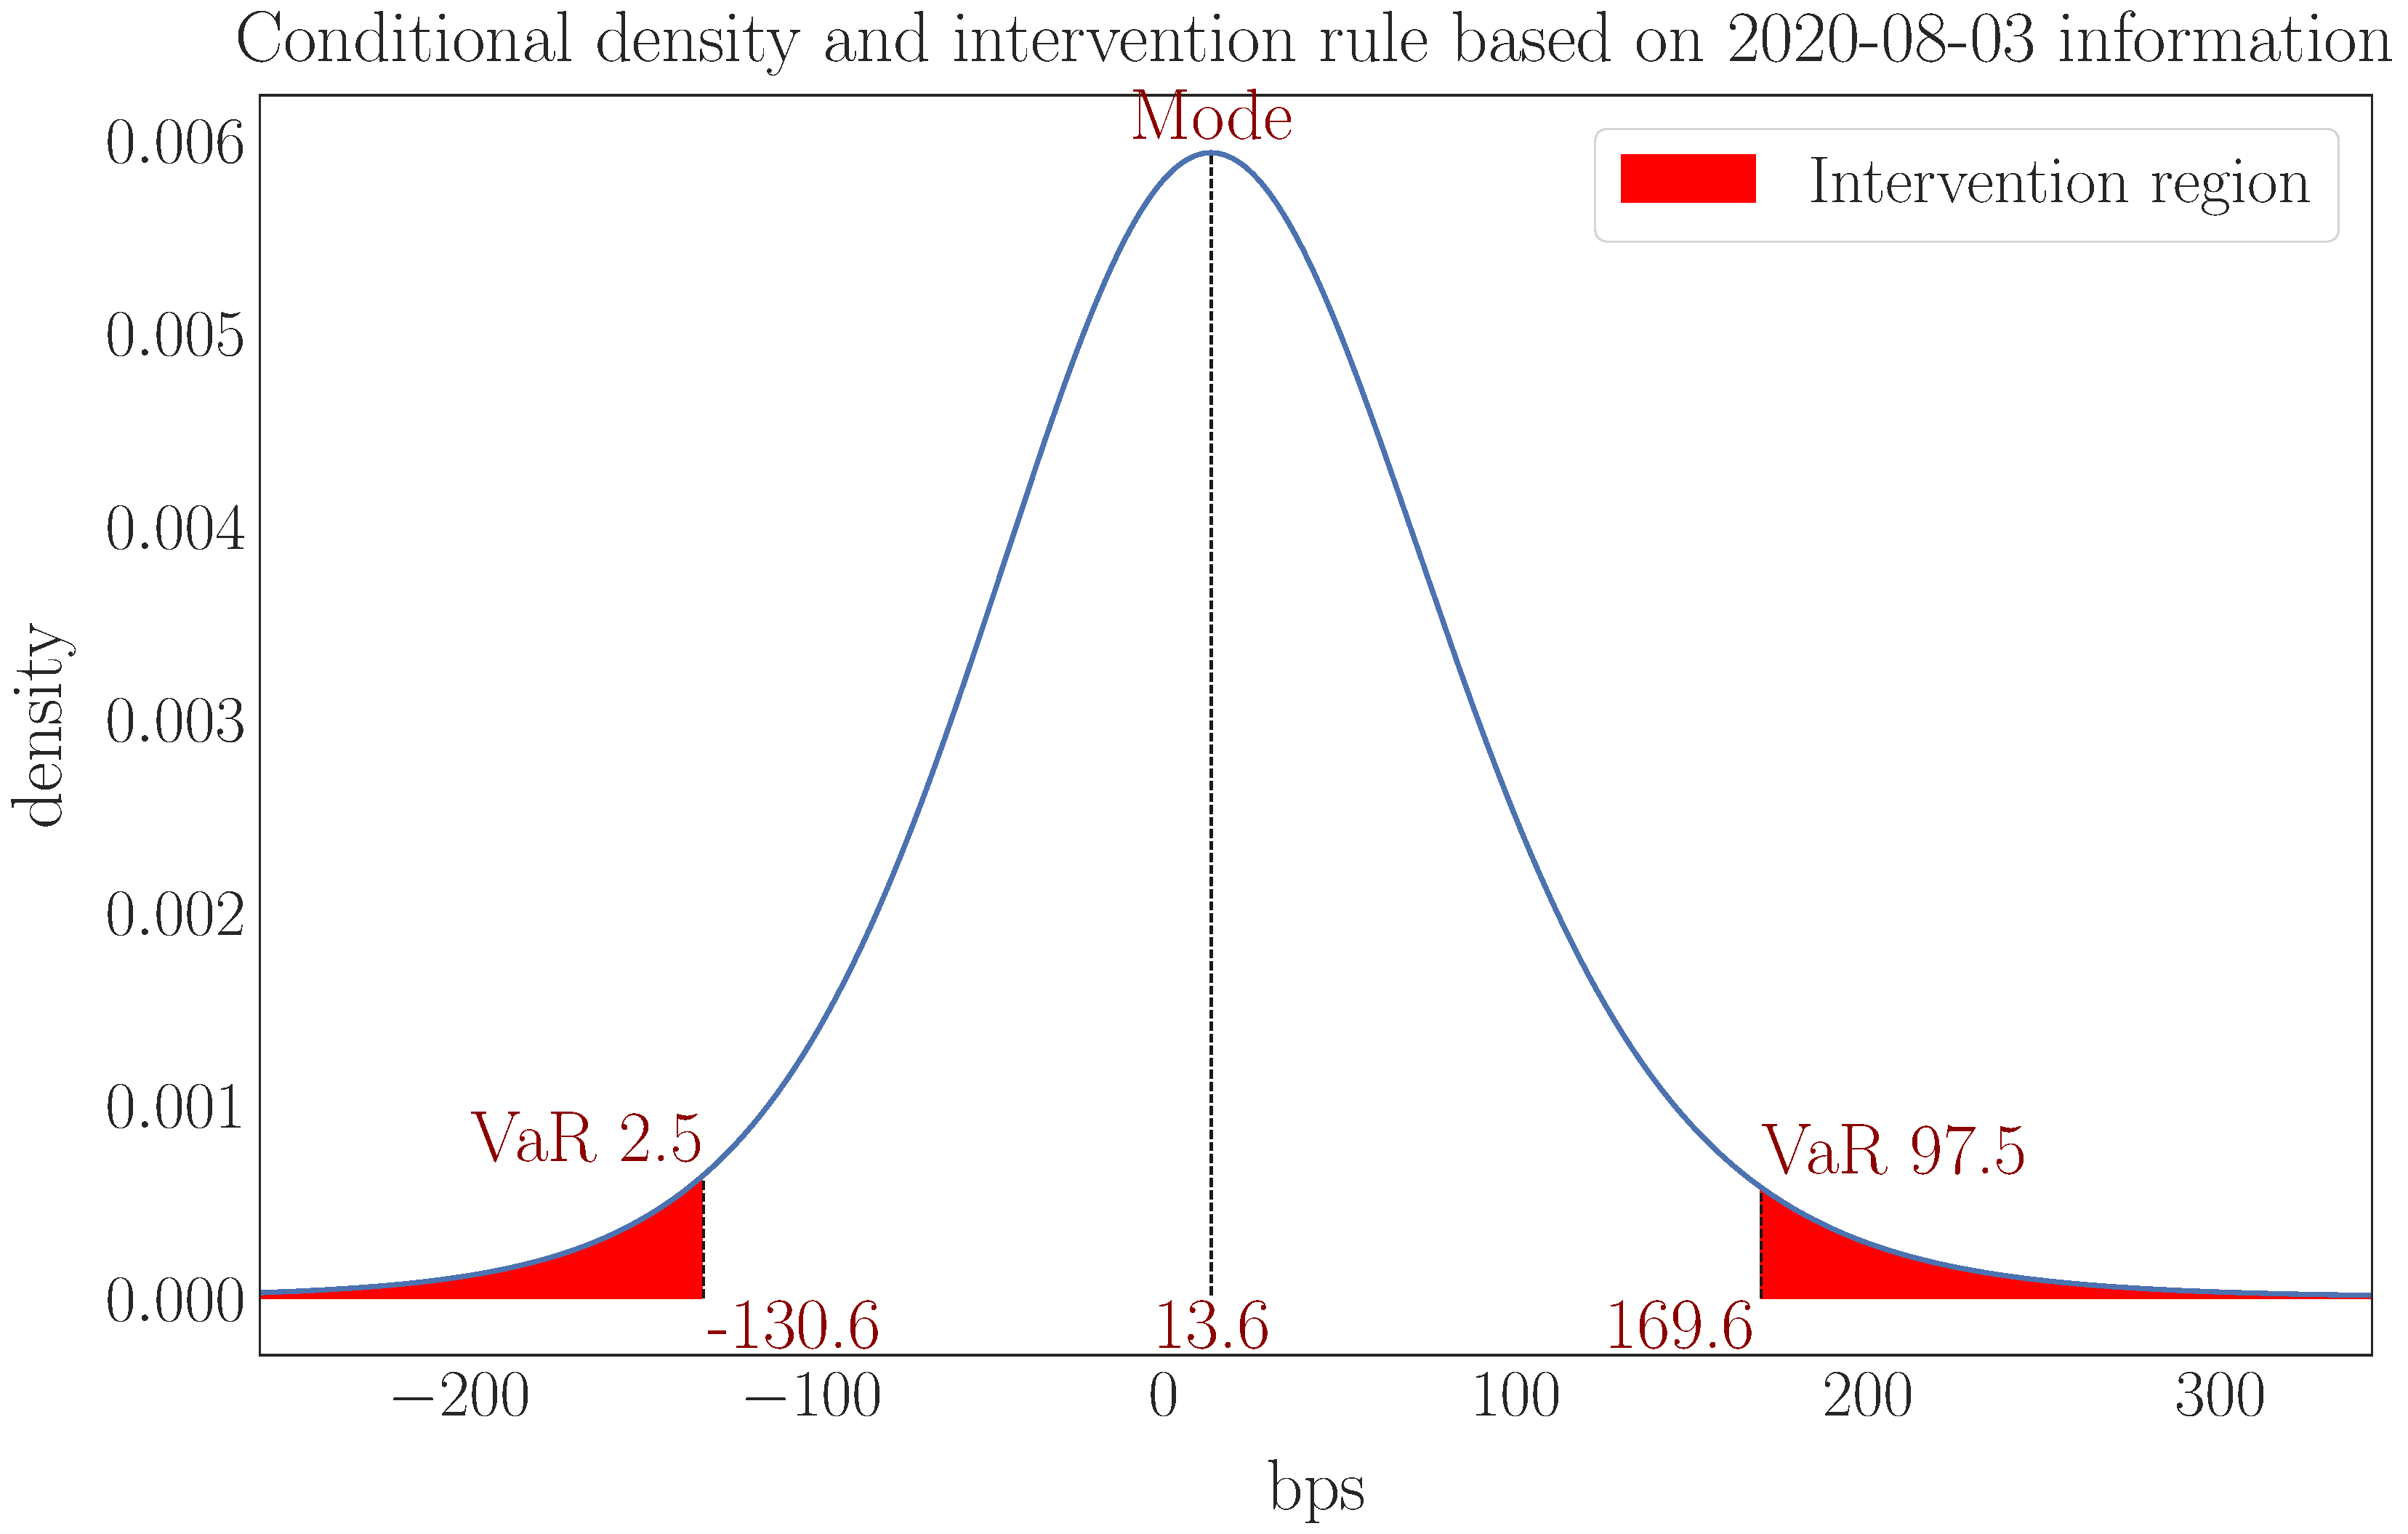
\includegraphics[width=\paperwidth]{var_rule.pdf}}
\end{frame}


%% ---------------------------------------------------------------------------
%% Model
%% ---------------------------------------------------------------------------
\section{Model}

\begin{frame}{Specification}

 \end{frame}


\begin{frame}{Regression Table}
\setlength\tabcolsep{2pt}  % default value: 6pt
\tiny  %%  command to change the font size
\begin{tabular}{llllll}
\toprule
{} & Microstructure &       CIP & Dollar move & Risk Appetite &  Baseline \\
\midrule
Intercept                       &       -2.33*** &     -2.29 &       -1.84 &         -2.55 &     -1.63 \\
Lag FX log returns              &       -0.07*** &     -0.08 &    -0.08*** &      -0.08*** &  -0.08*** \\
Bid ask abs                     &           5.71 &     24.39 &      -35.66 &         -2.42 &      3.23 \\
Min max abs                     &       35.56*** &     34.63 &       34.32 &        34.55* &     26.21 \\
Forward points first difference &       23.29*** &  17.79*** &    26.44*** &       19.8*** &  19.44*** \\
Interbank rate vs Libor         &                &  33.61*** &    39.32*** &      34.75*** &  33.86*** \\
EURUSD log returns              &                &           &    -0.14*** &      -0.17*** &  -0.16*** \\
VIX first diff                  &                &           &             &      15.66*** &  15.37*** \\
FX intervention dummy lag       &                &           &             &               &      2.23 \\
Oil prices log returns          &                &           &             &               &  -0.02*** \\
Omega                           &        0.13*** &      0.13 &     0.12*** &       0.11*** &   0.12*** \\
Alpha                           &        0.17*** &     0.17* &     0.16*** &       0.16*** &   0.15*** \\
Gamma                           &        0.07*** &   0.06*** &     0.06*** &       0.05*** &   0.05*** \\
Beta                            &        0.98*** &   0.99*** &     0.99*** &       0.99*** &   0.99*** \\
Nu                              &        8.33*** &   8.66*** &     8.92*** &       8.71*** &   8.54*** \\
Lambda                          &        0.08*** &      0.07 &        0.09 &         0.07* &   0.08*** \\
R2                              &          5.8 \% &     6.7 \% &      10.4 \% &        27.3 \% &    27.6 \% \\
R2 adjusted                     &          5.8 \% &     6.6 \% &      10.4 \% &        27.2 \% &    27.5 \% \\
Number of observations          &           5986 &      5986 &        5682 &          5682 &      5680 \\
Significance *10\%, **5\%, ***1\%  &                &           &             &               &           \\
\bottomrule
\end{tabular}

\normalsize
\end{frame}


%% ---------------------------------------------------------------------------
%% In-sample dynamics
%% ---------------------------------------------------------------------------
\section{In-sample dynamics}
\begin{frame}
\frametitle{Dynamics of the Mexican Peso against USD}
    \makebox[\linewidth]{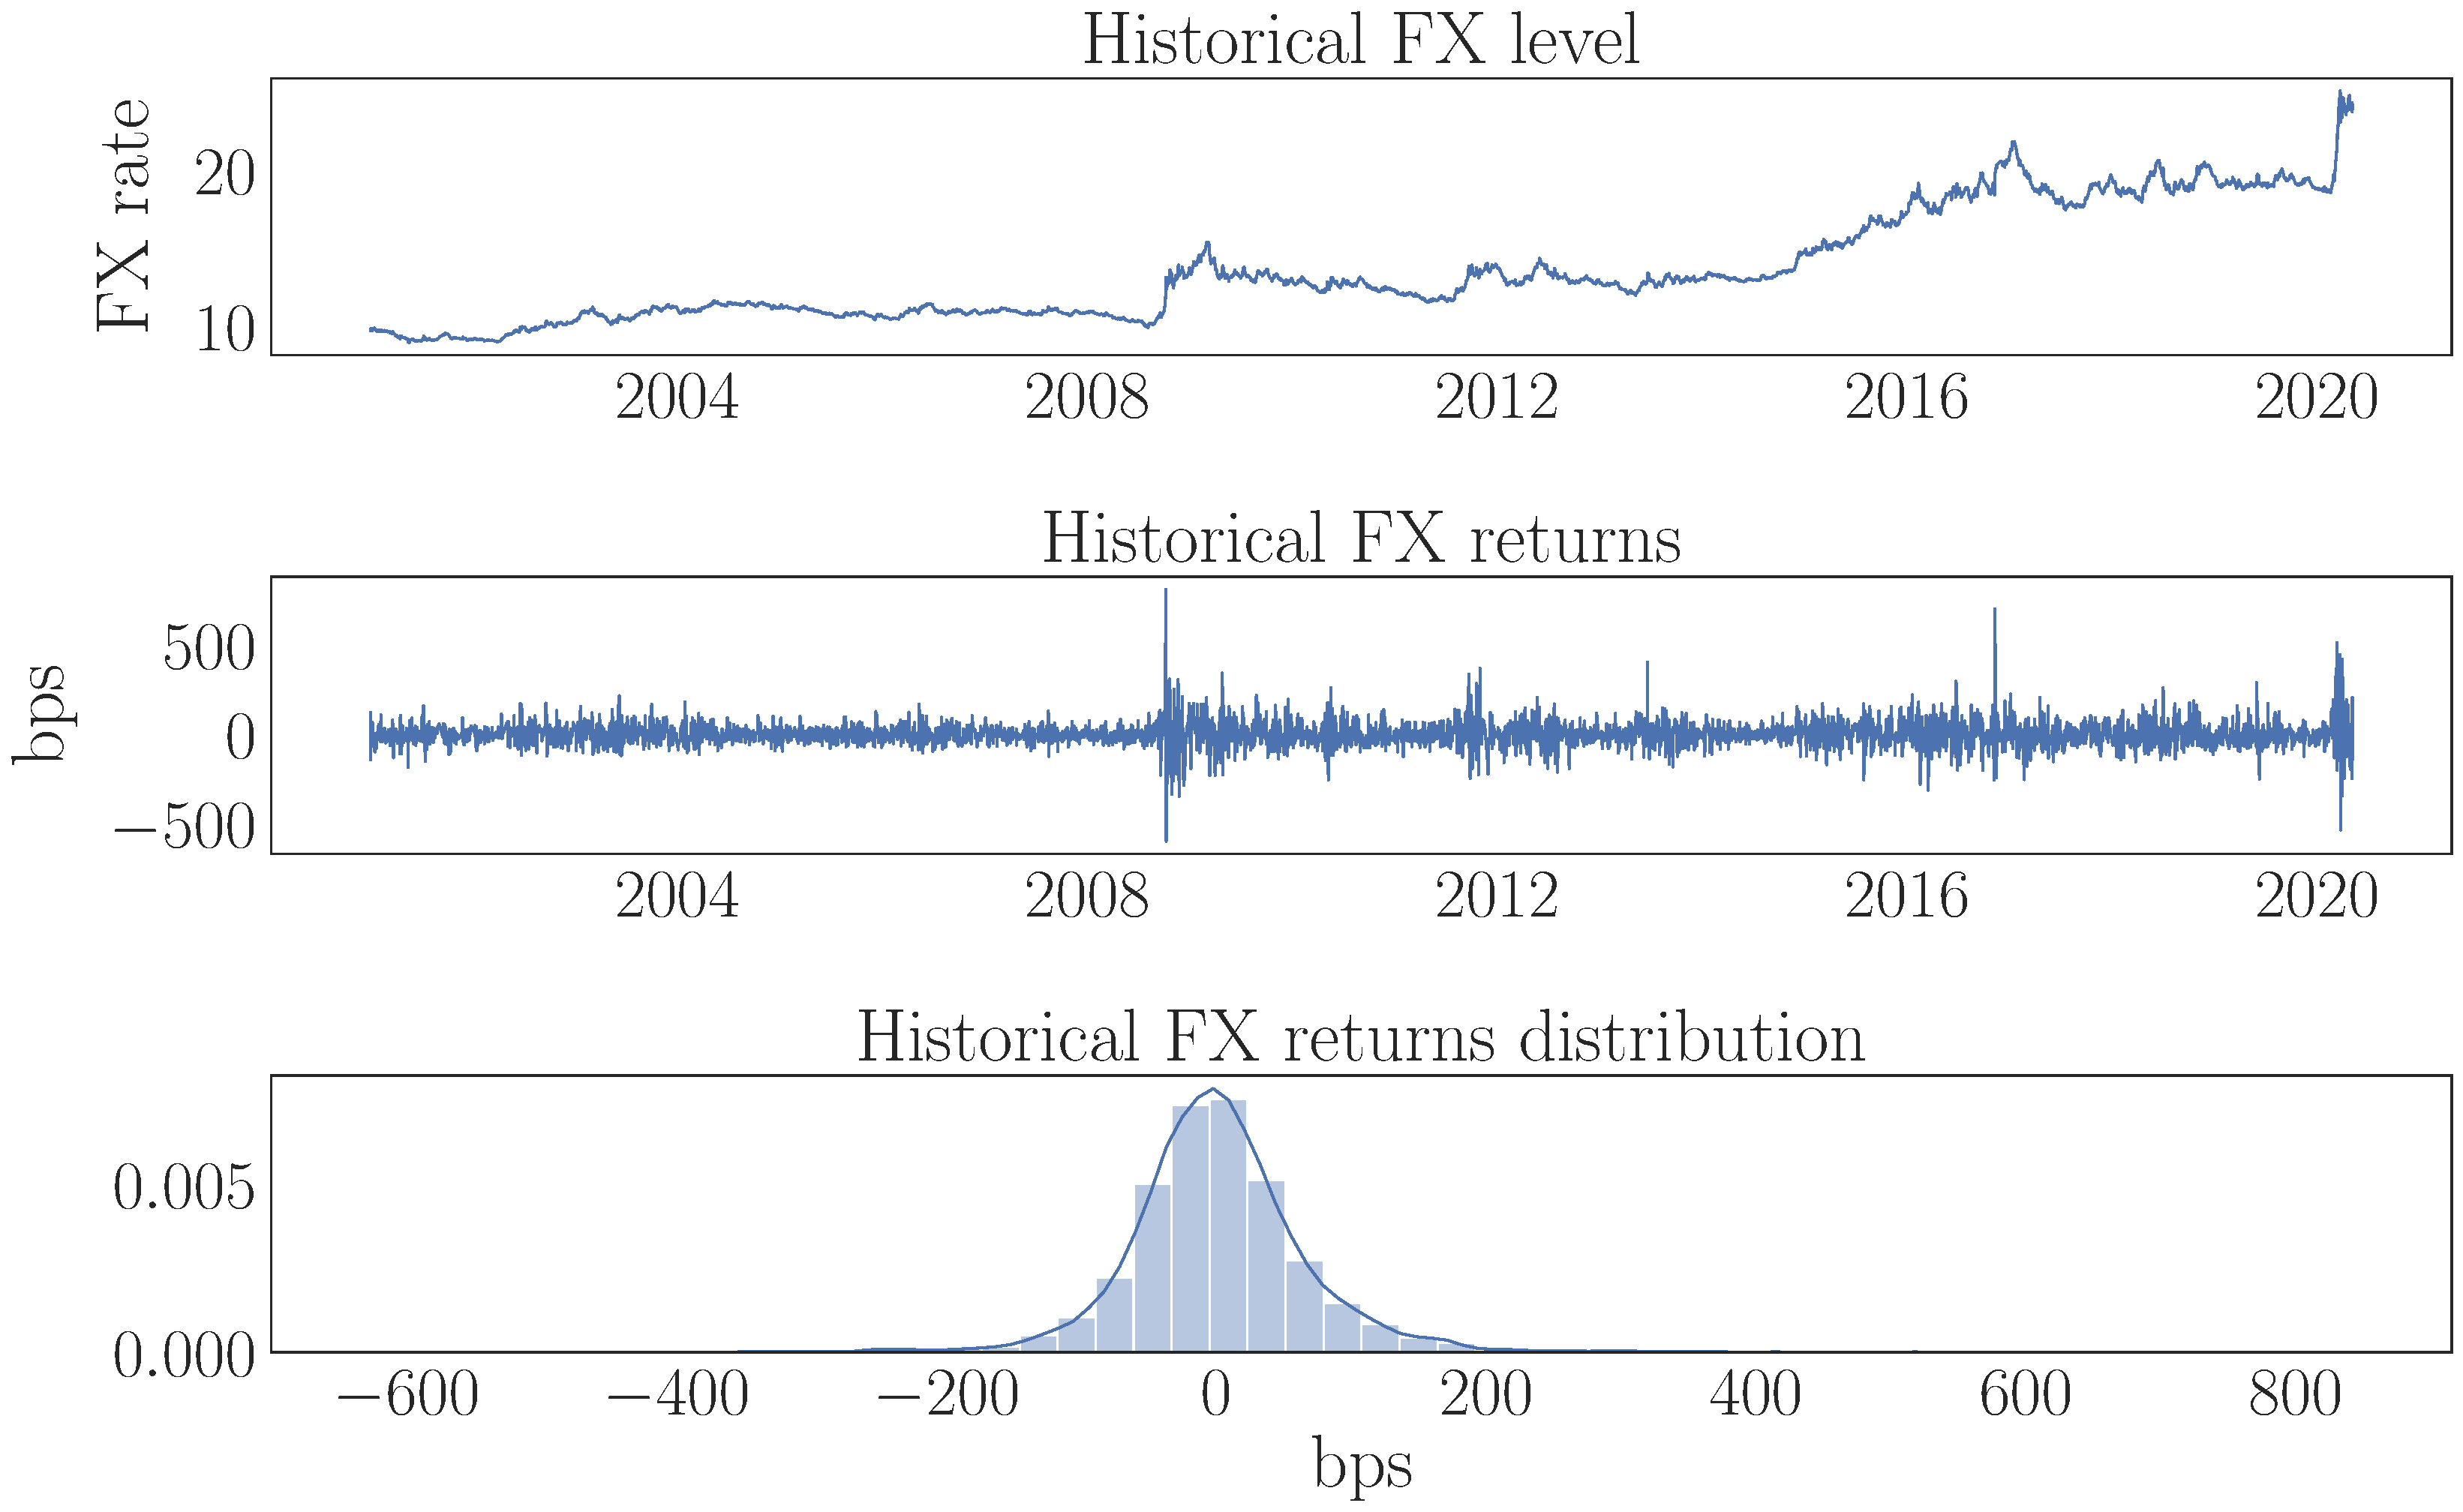
\includegraphics[width=\paperwidth]{descriptive_plot.pdf}}
\end{frame}


\begin{frame}
\frametitle{Conditional In-Sample Volatility of the Mexican Peso}
    \makebox[\linewidth]{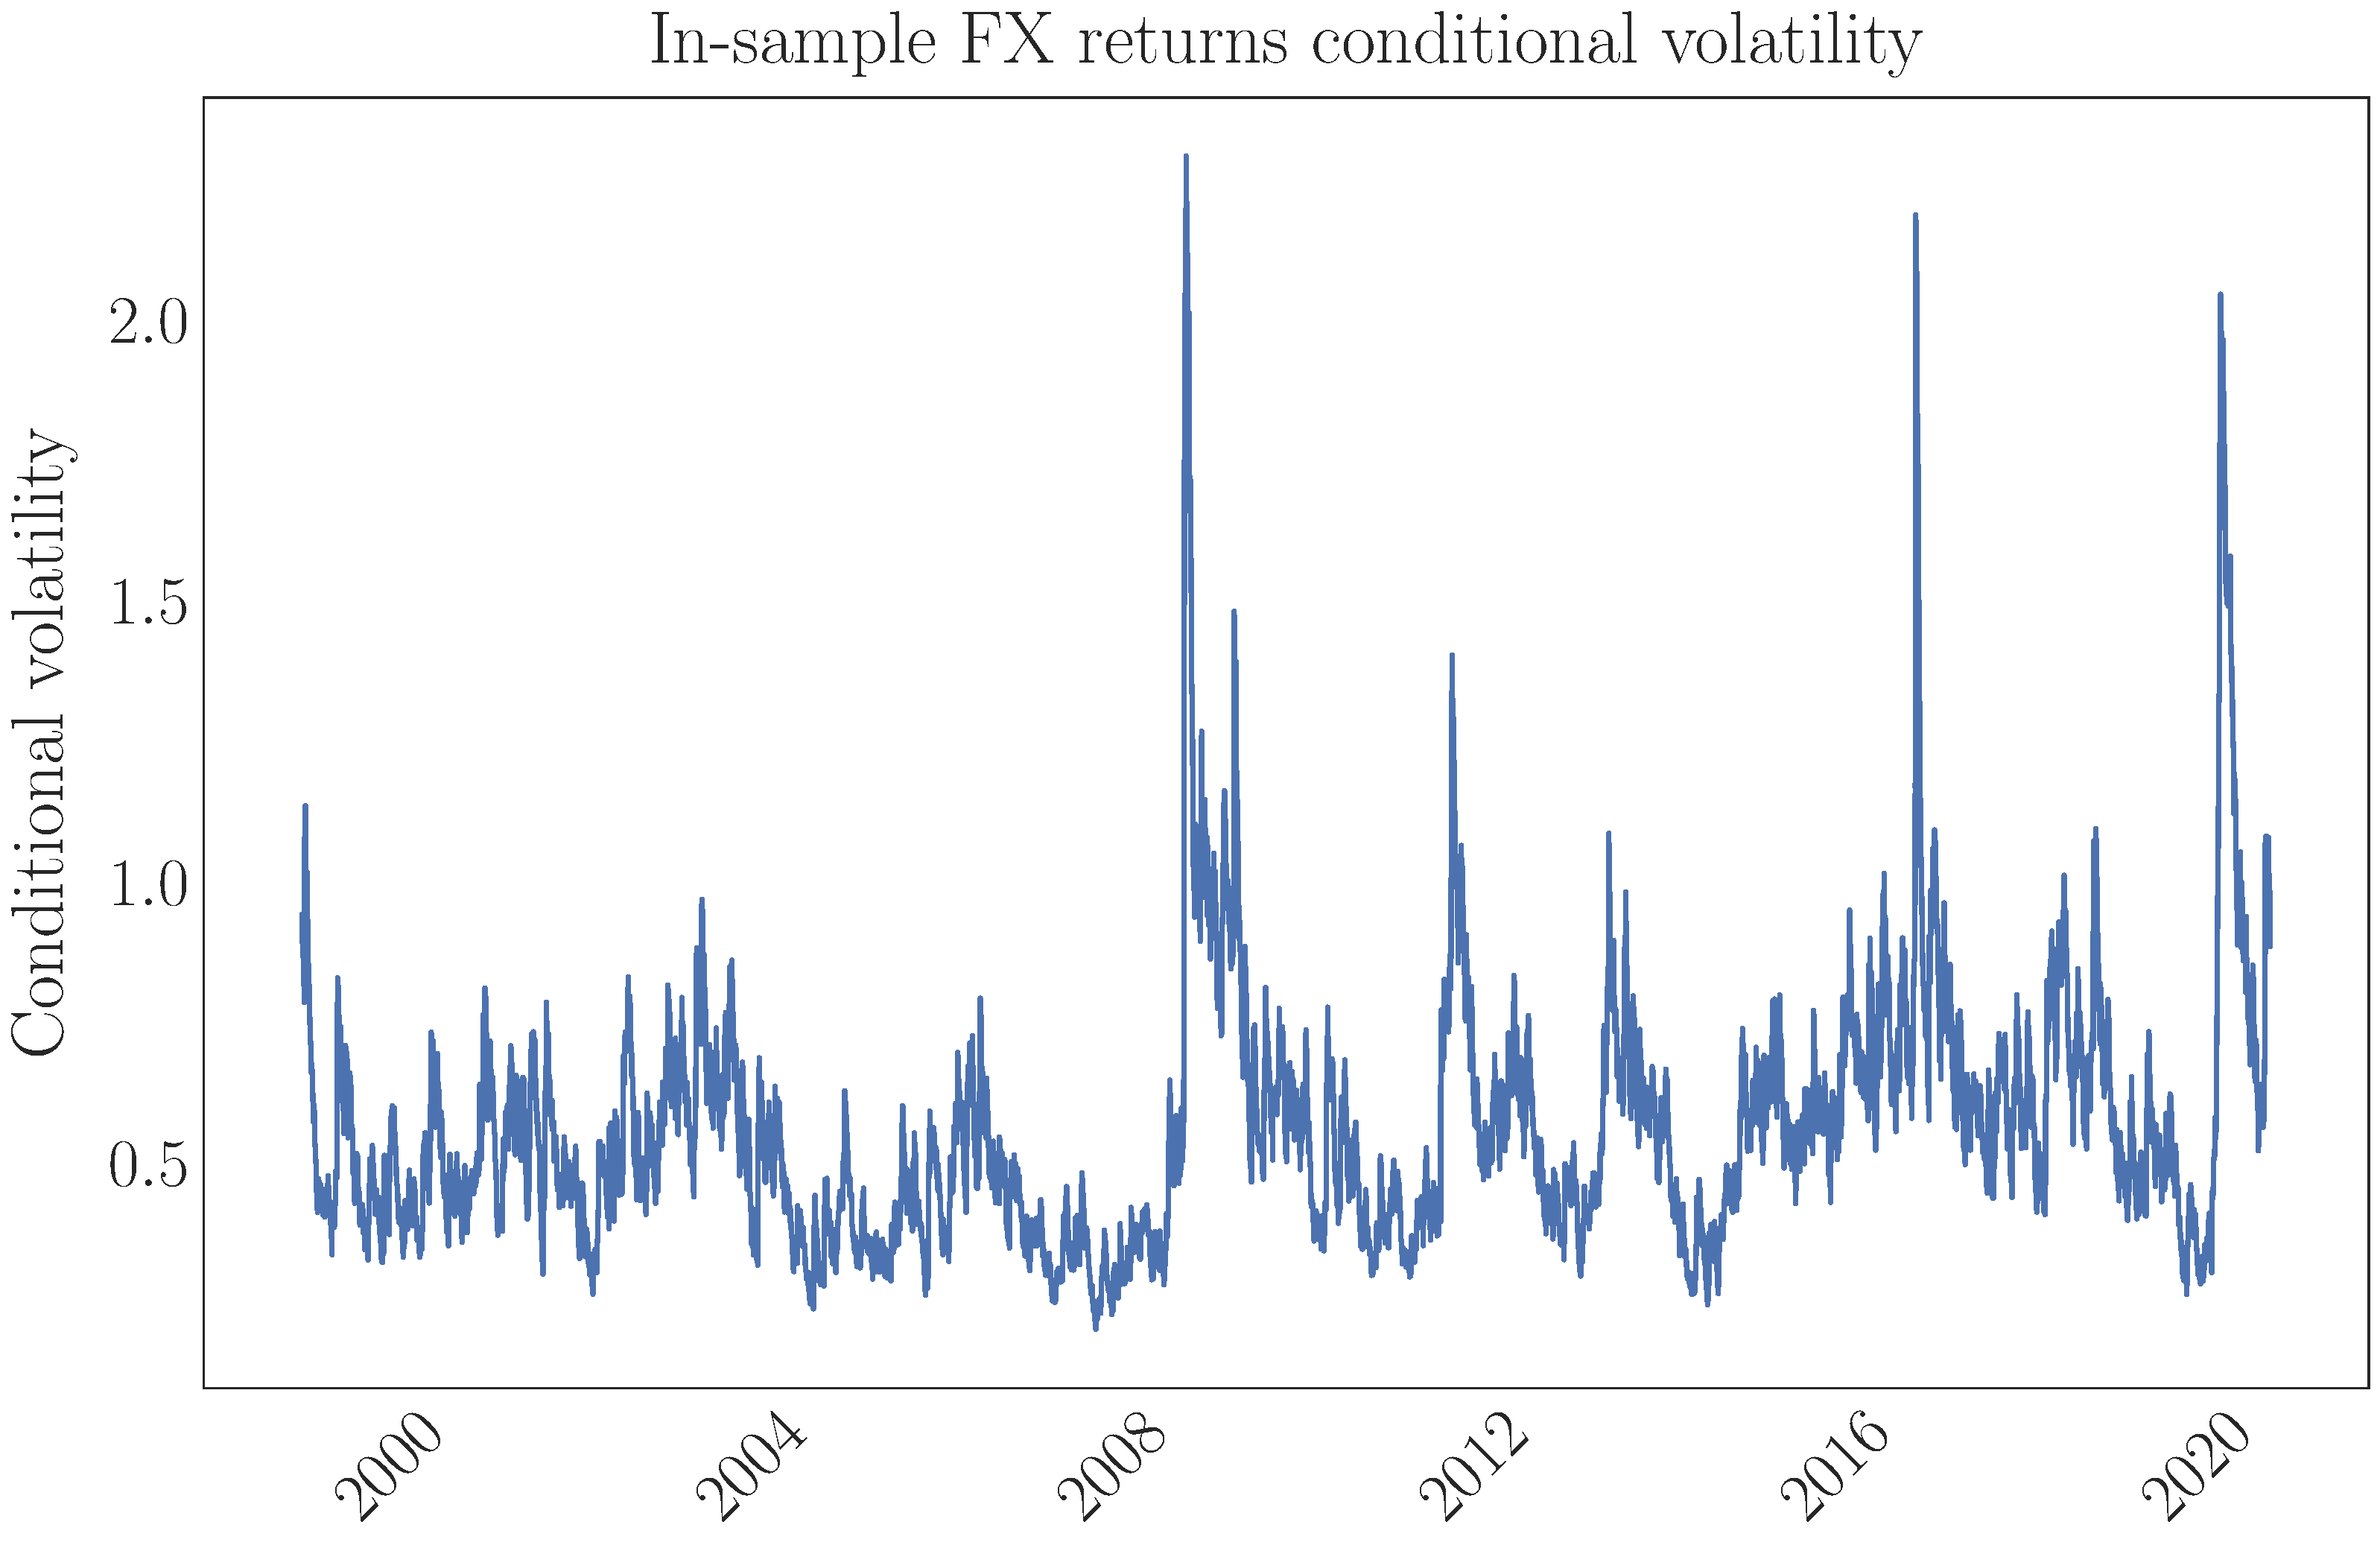
\includegraphics[width=\paperwidth]{conditional_vol_plot.pdf}}
\end{frame}

%% ---------------------------------------------------------------------------
%% Forecasting
%% ---------------------------------------------------------------------------
\section{Forecasting}
\begin{frame}
 %\frametitle{Conditional Distributions}
\makebox[\linewidth]{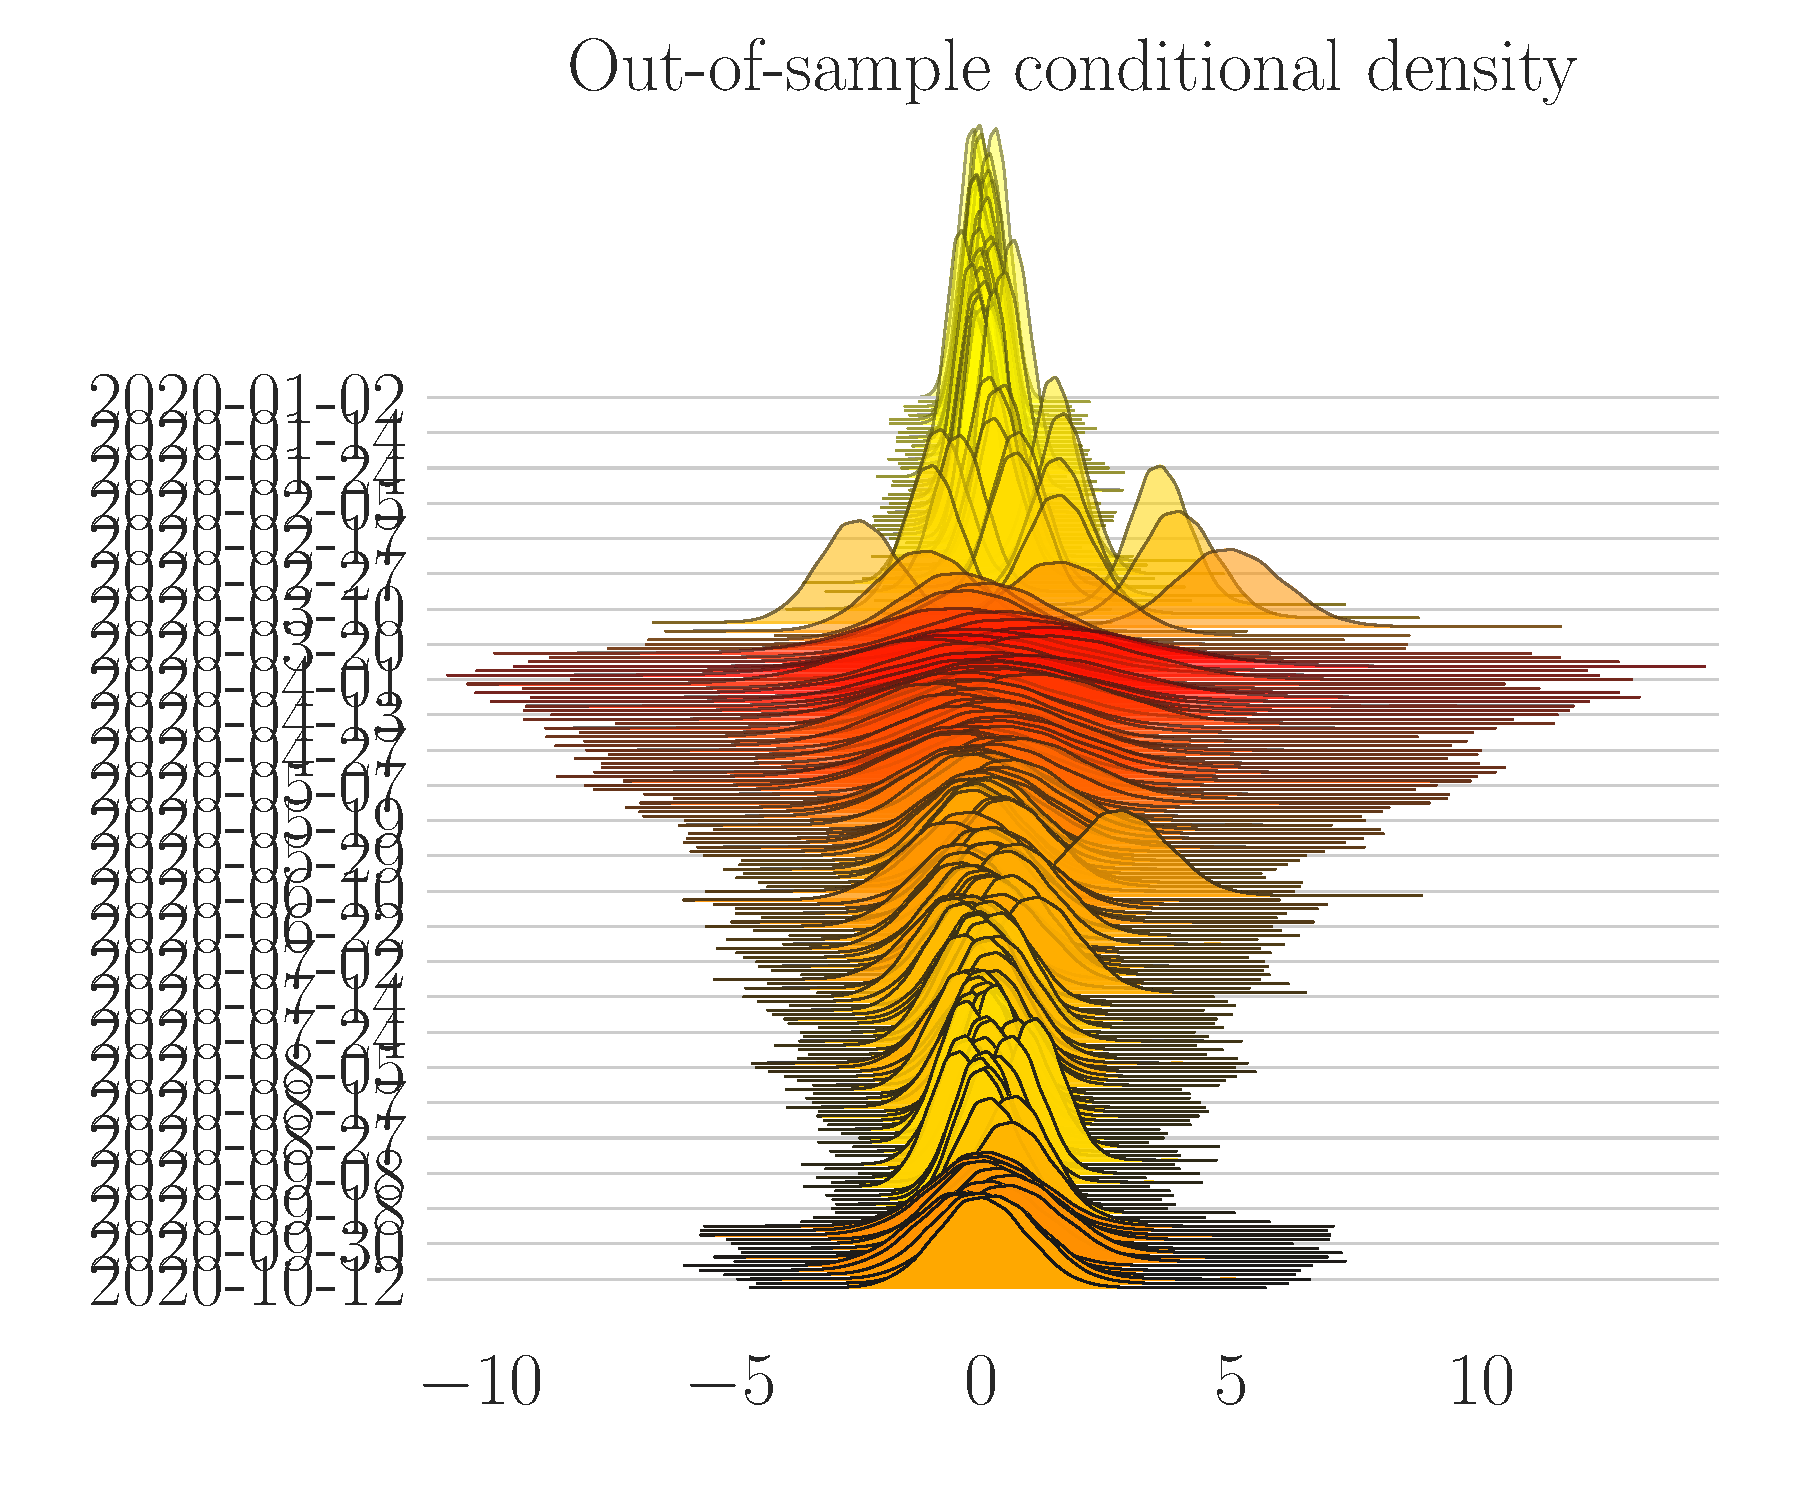
\includegraphics[width=\paperwidth, height=\paperheight]{joyplot.pdf}}
\end{frame}

\begin{frame}
 \frametitle{Fan Chart}
\makebox[\linewidth]{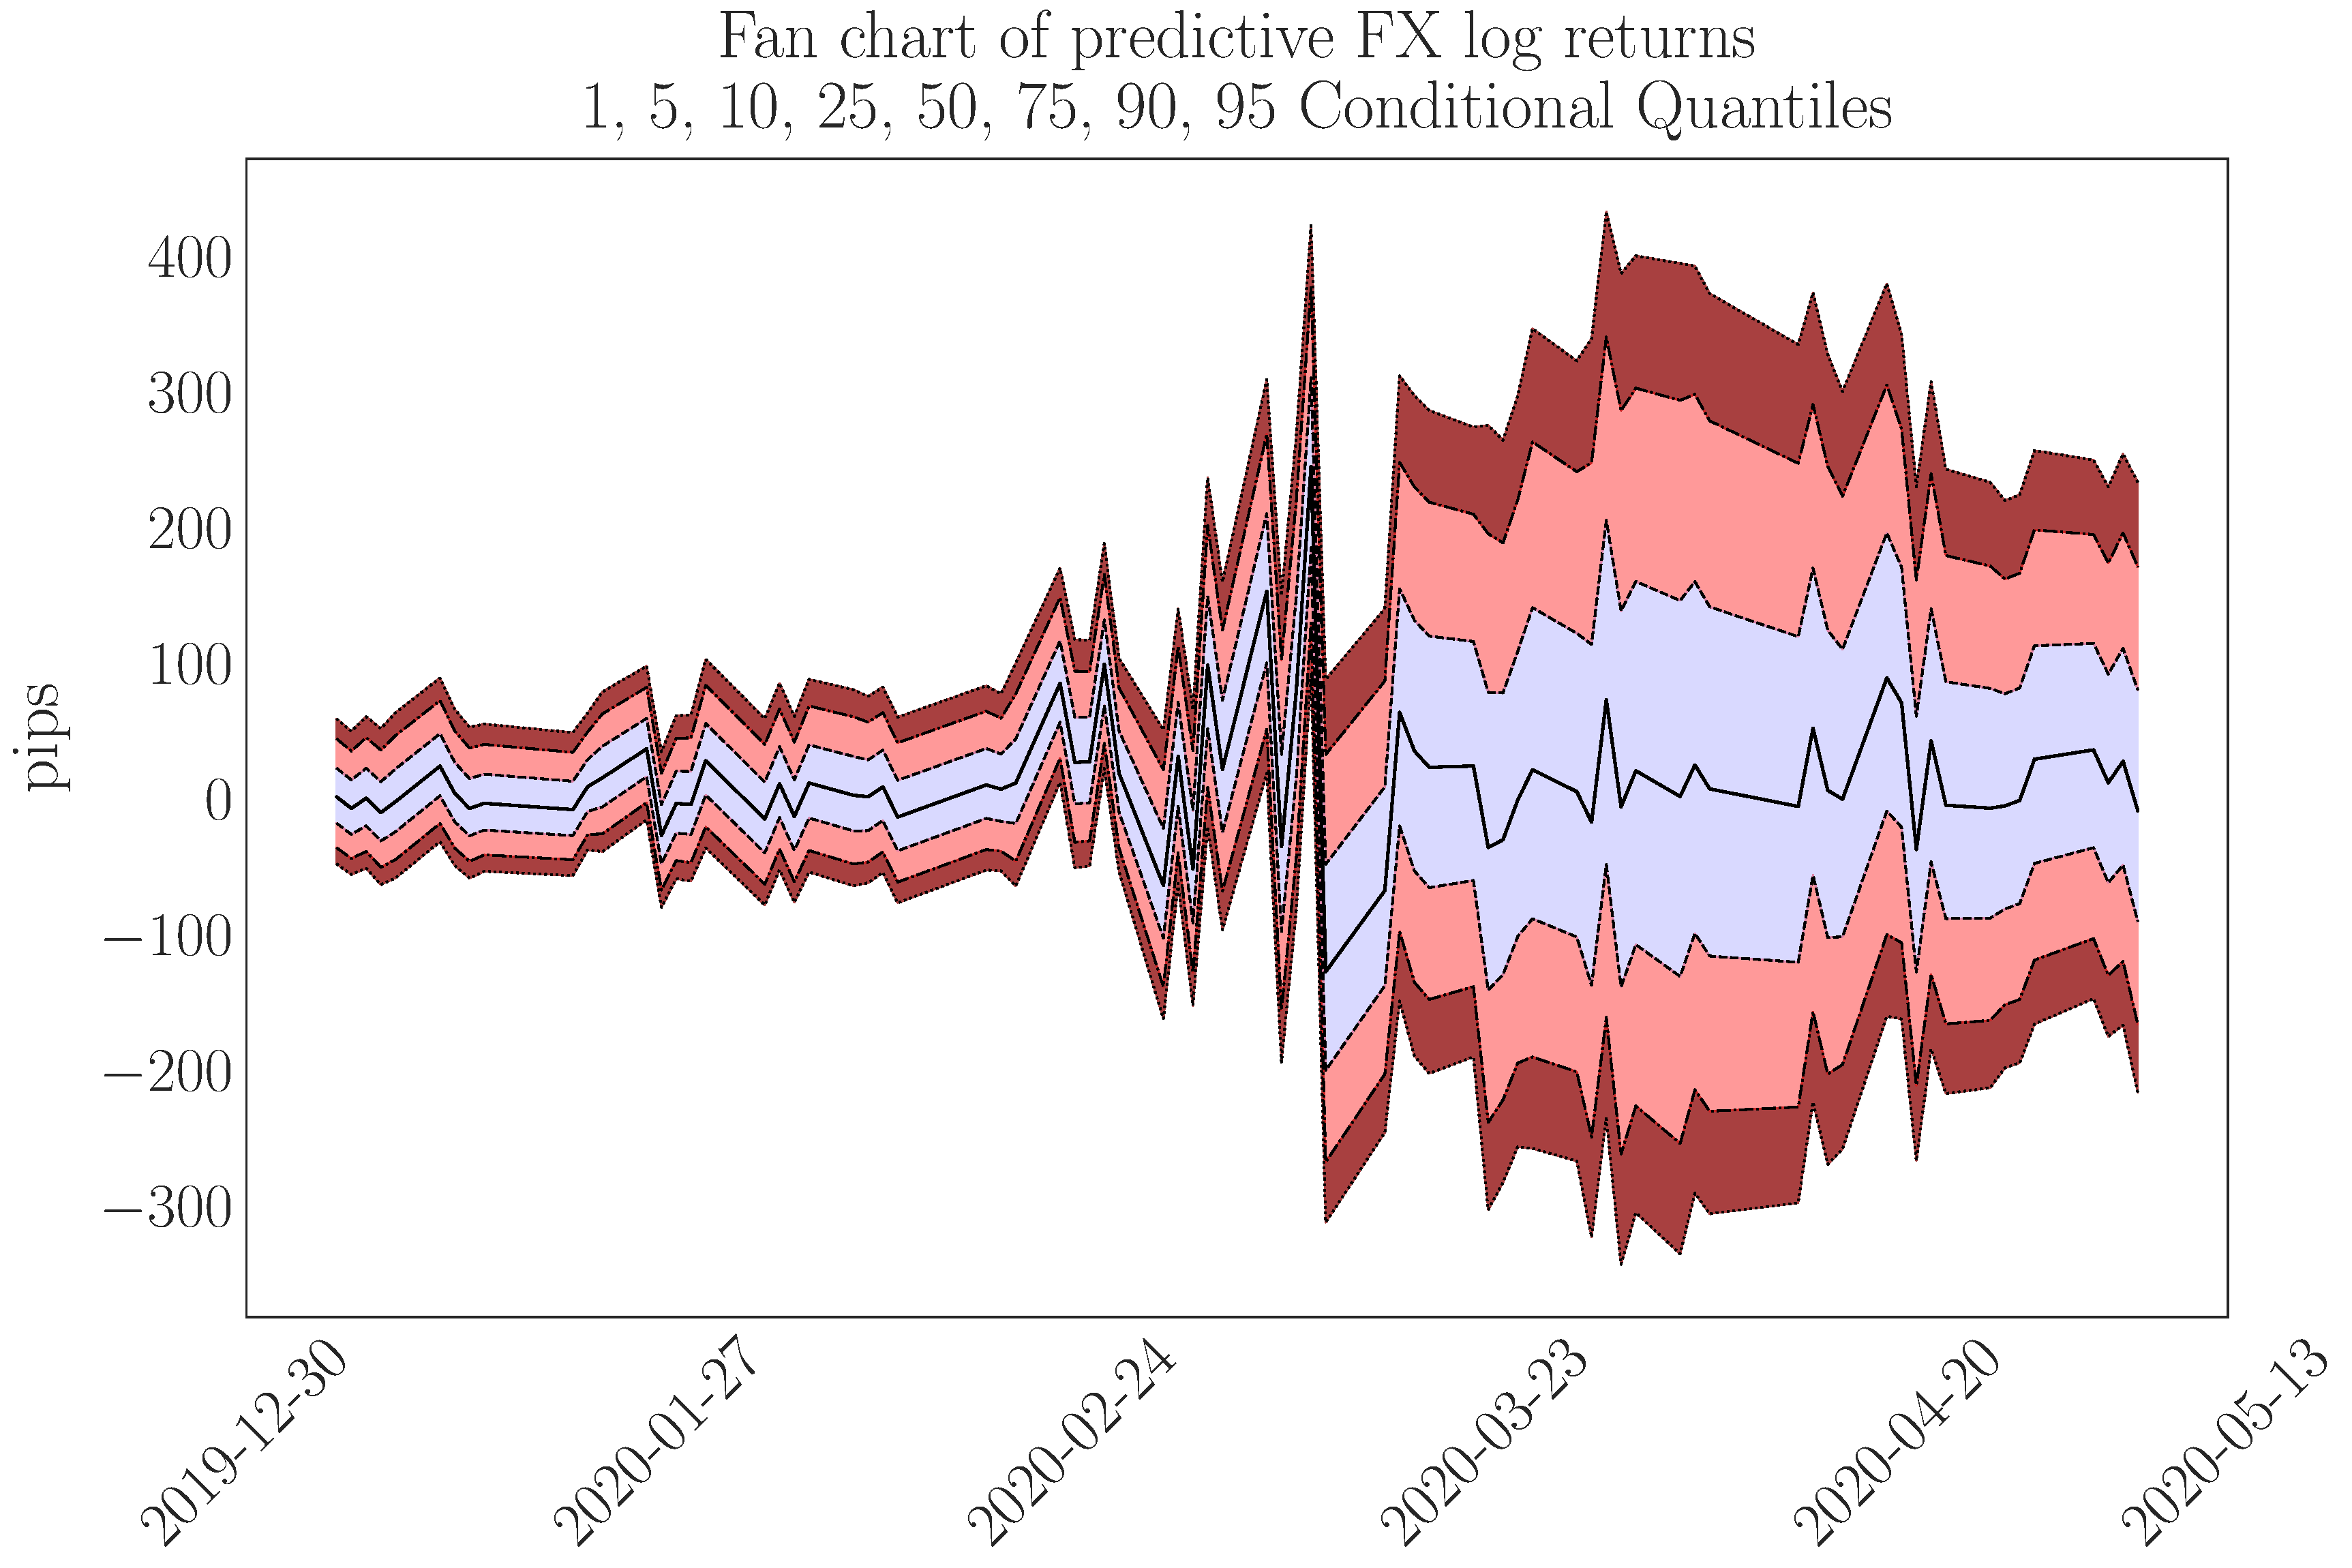
\includegraphics[width=0.95\paperwidth]{fanchart.pdf}}
\end{frame}

\begin{frame}
  \frametitle{VaR FXI Rule}
    \makebox[\linewidth]{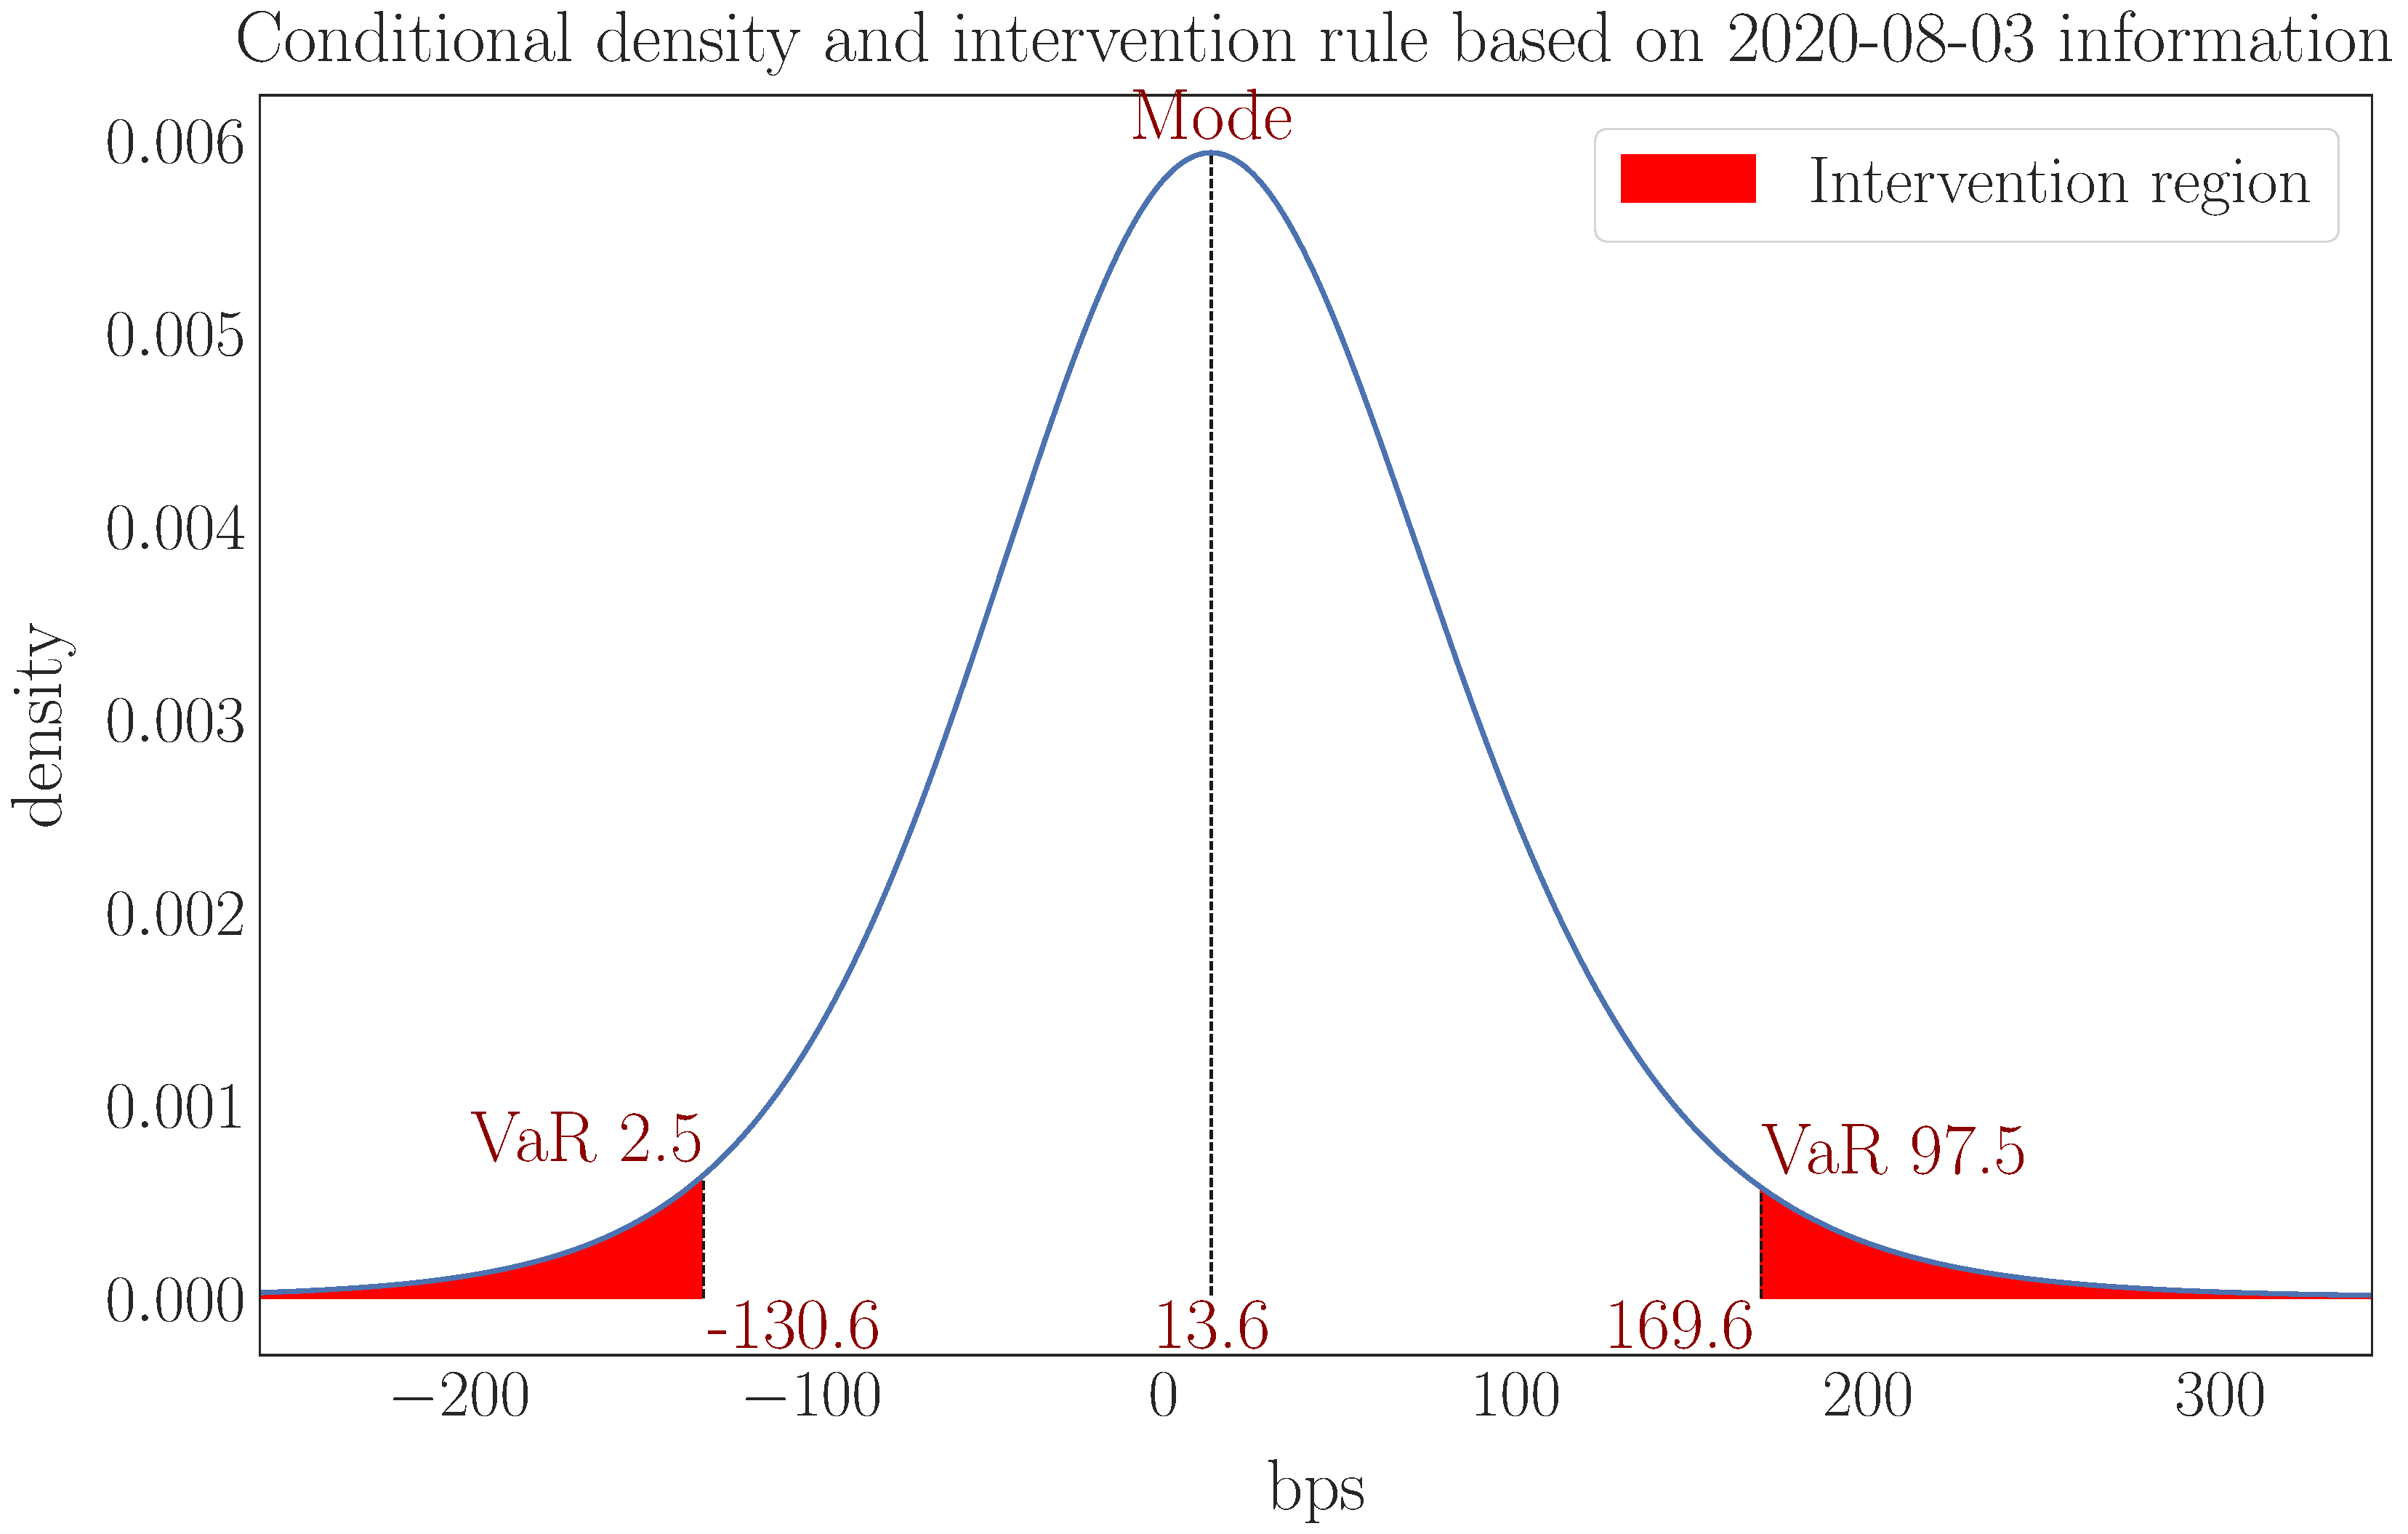
\includegraphics[width=\paperwidth]{var_rule.pdf}}
\end{frame}

\begin{frame}
  \frametitle{Conditional Cumulative Distribution Function}
    \makebox[\linewidth]{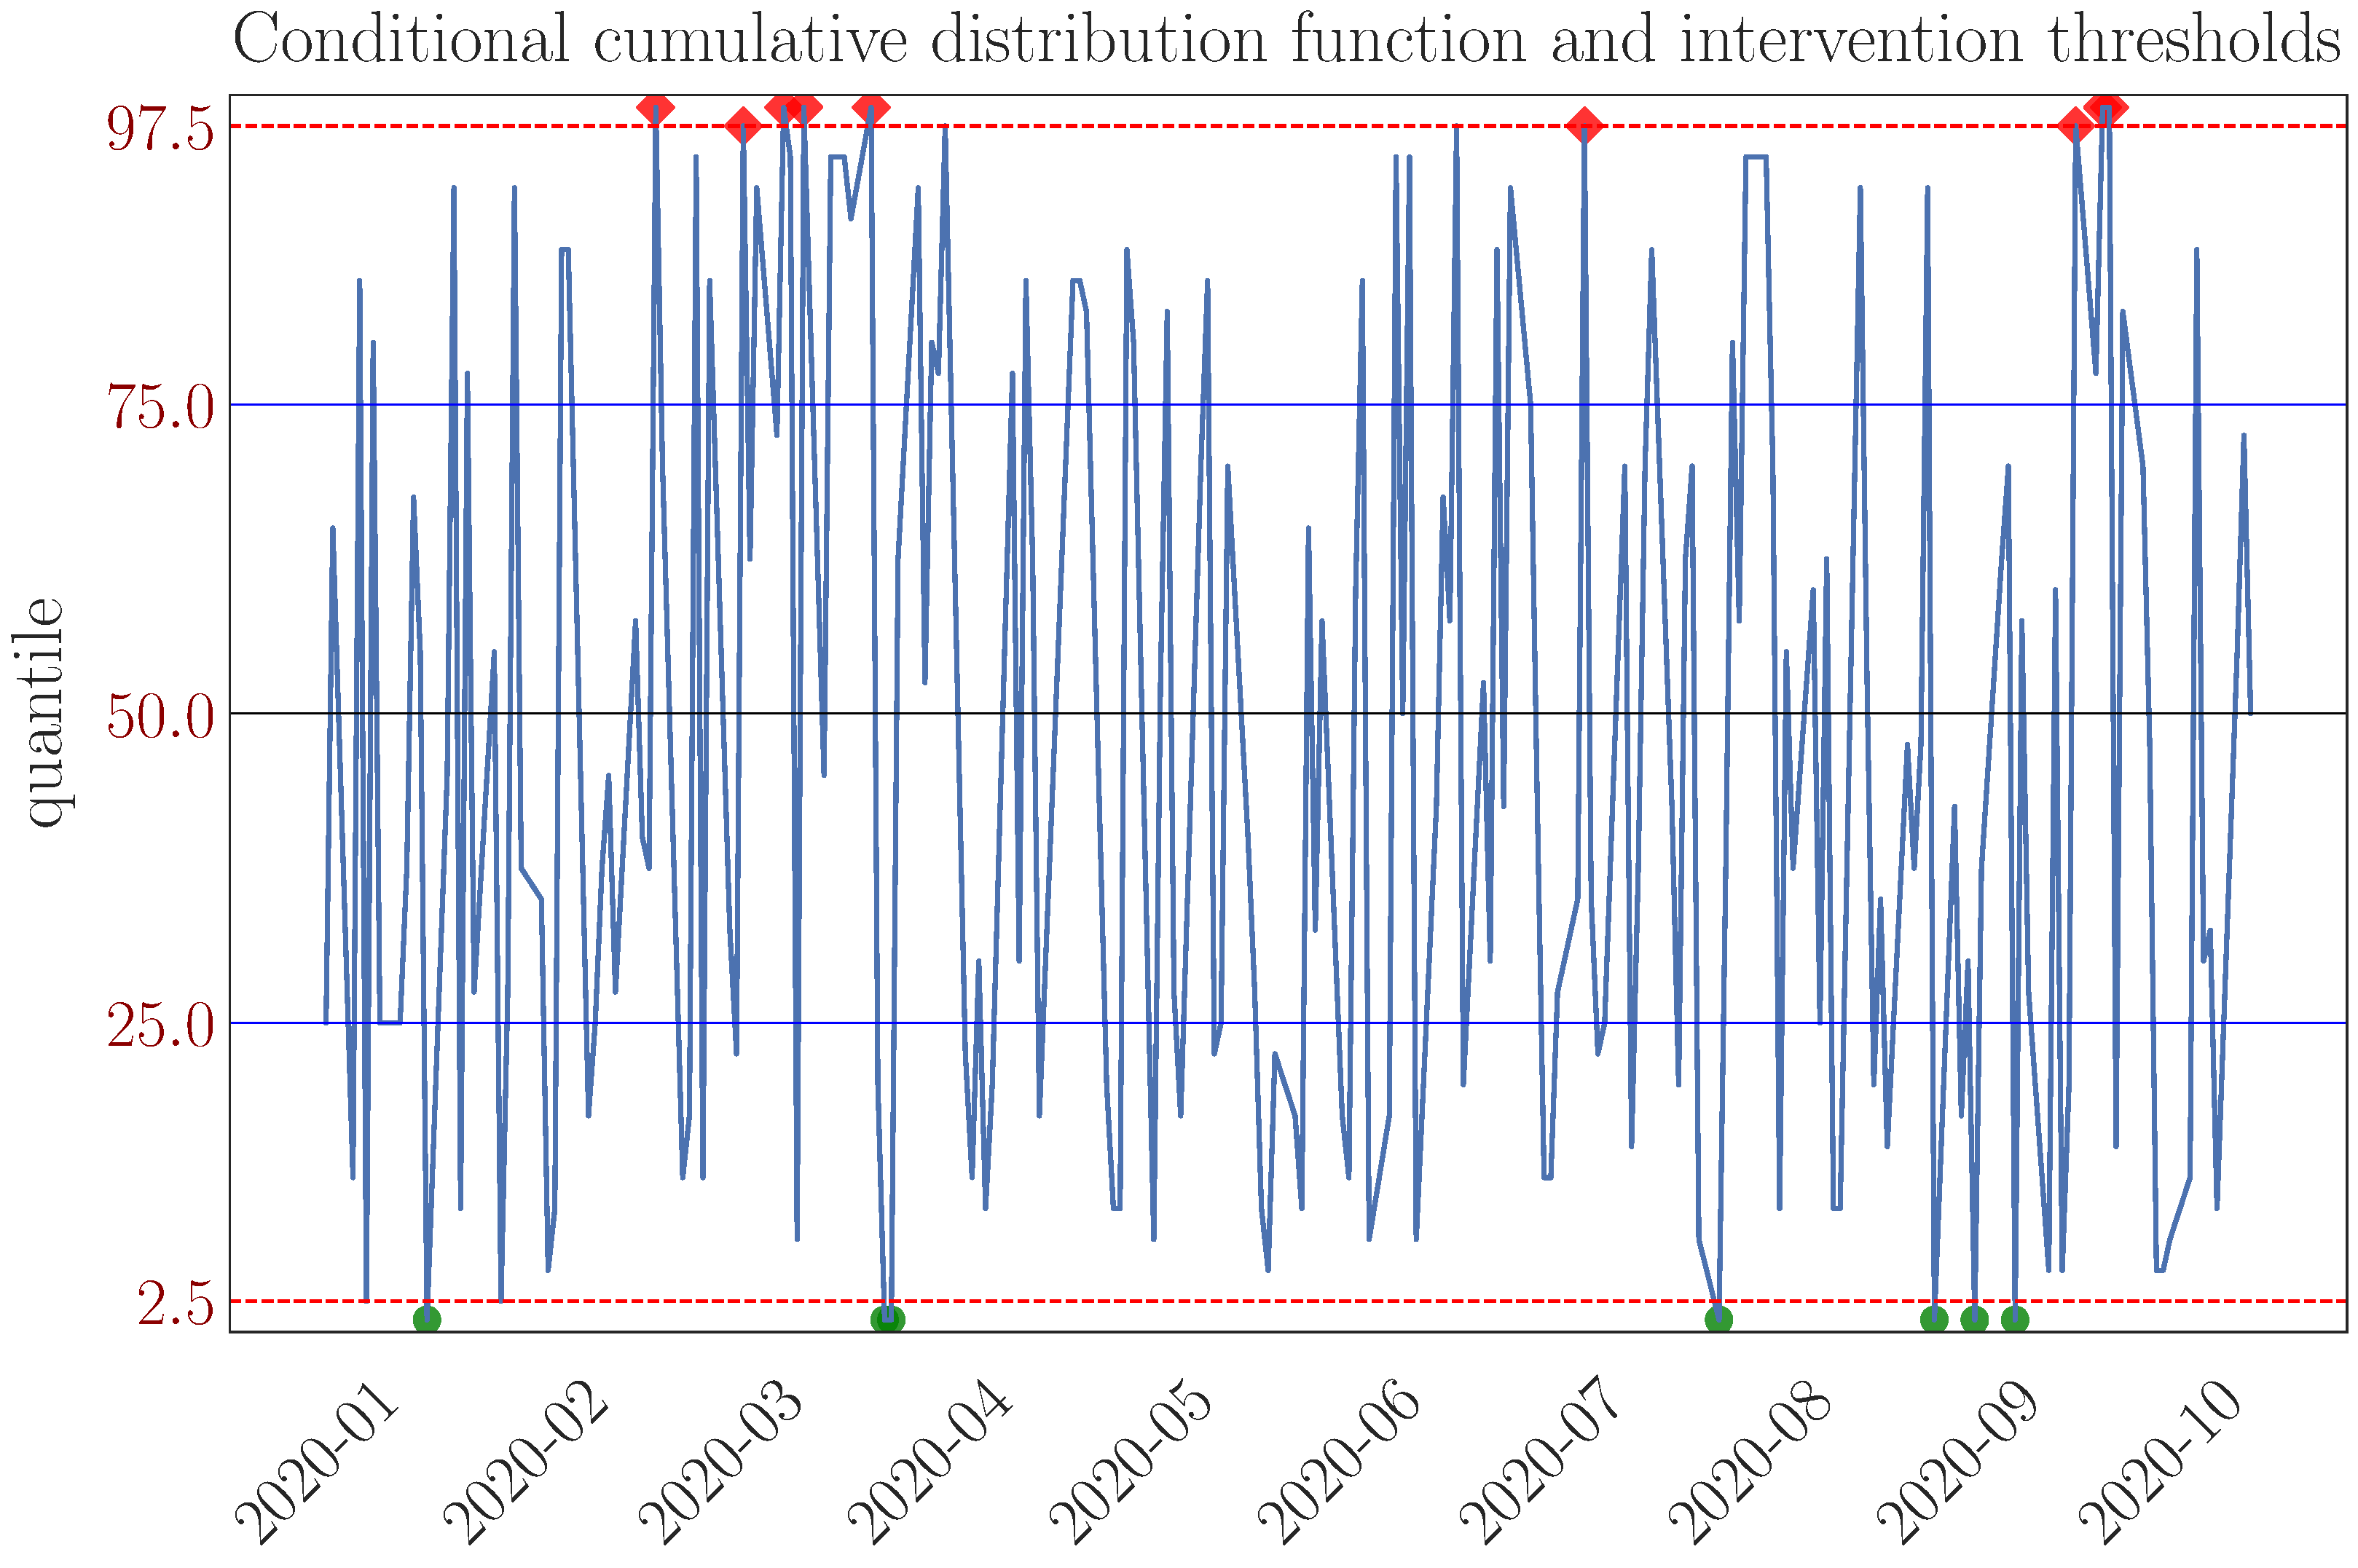
\includegraphics[width=\paperwidth]{conditional_cdf.pdf}}
\end{frame}

\begin{frame}
  \frametitle{Conditional Exceedance}
    \makebox[\linewidth]{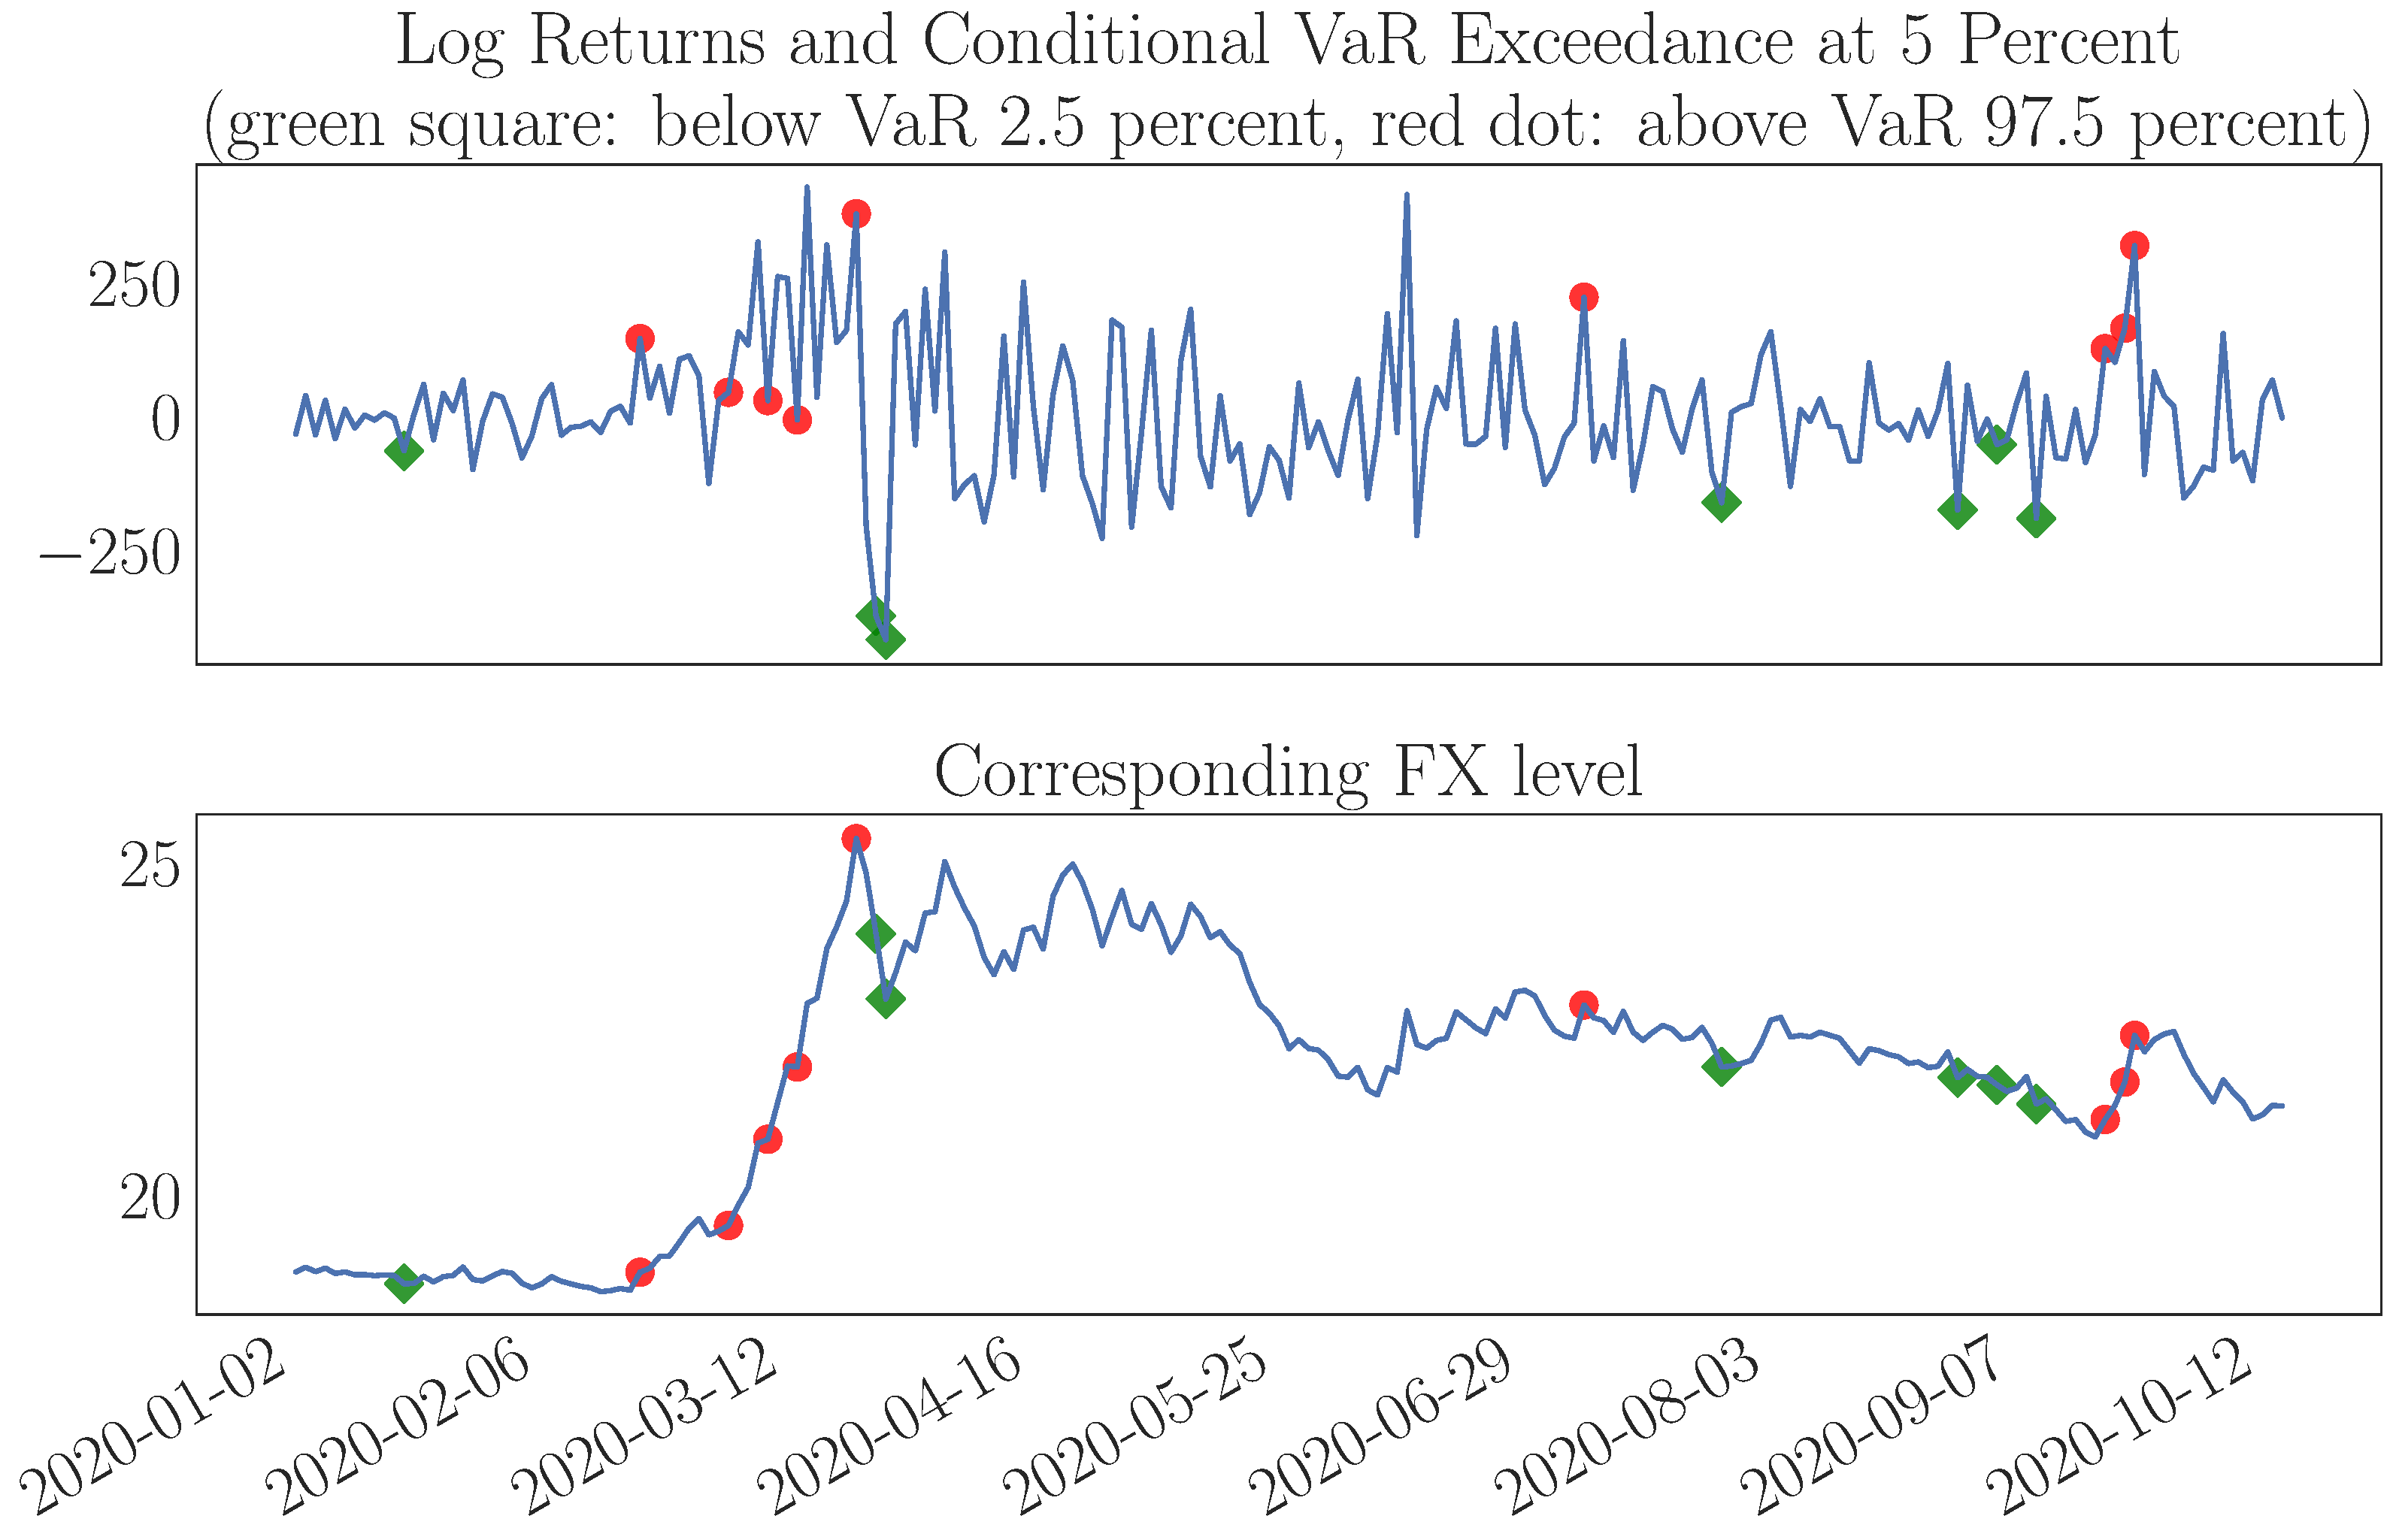
\includegraphics[width=\paperwidth]{conditional_exceedance.pdf}}
\end{frame}


\begin{frame}
  \frametitle{Density Evaluation}
    \makebox[\linewidth]{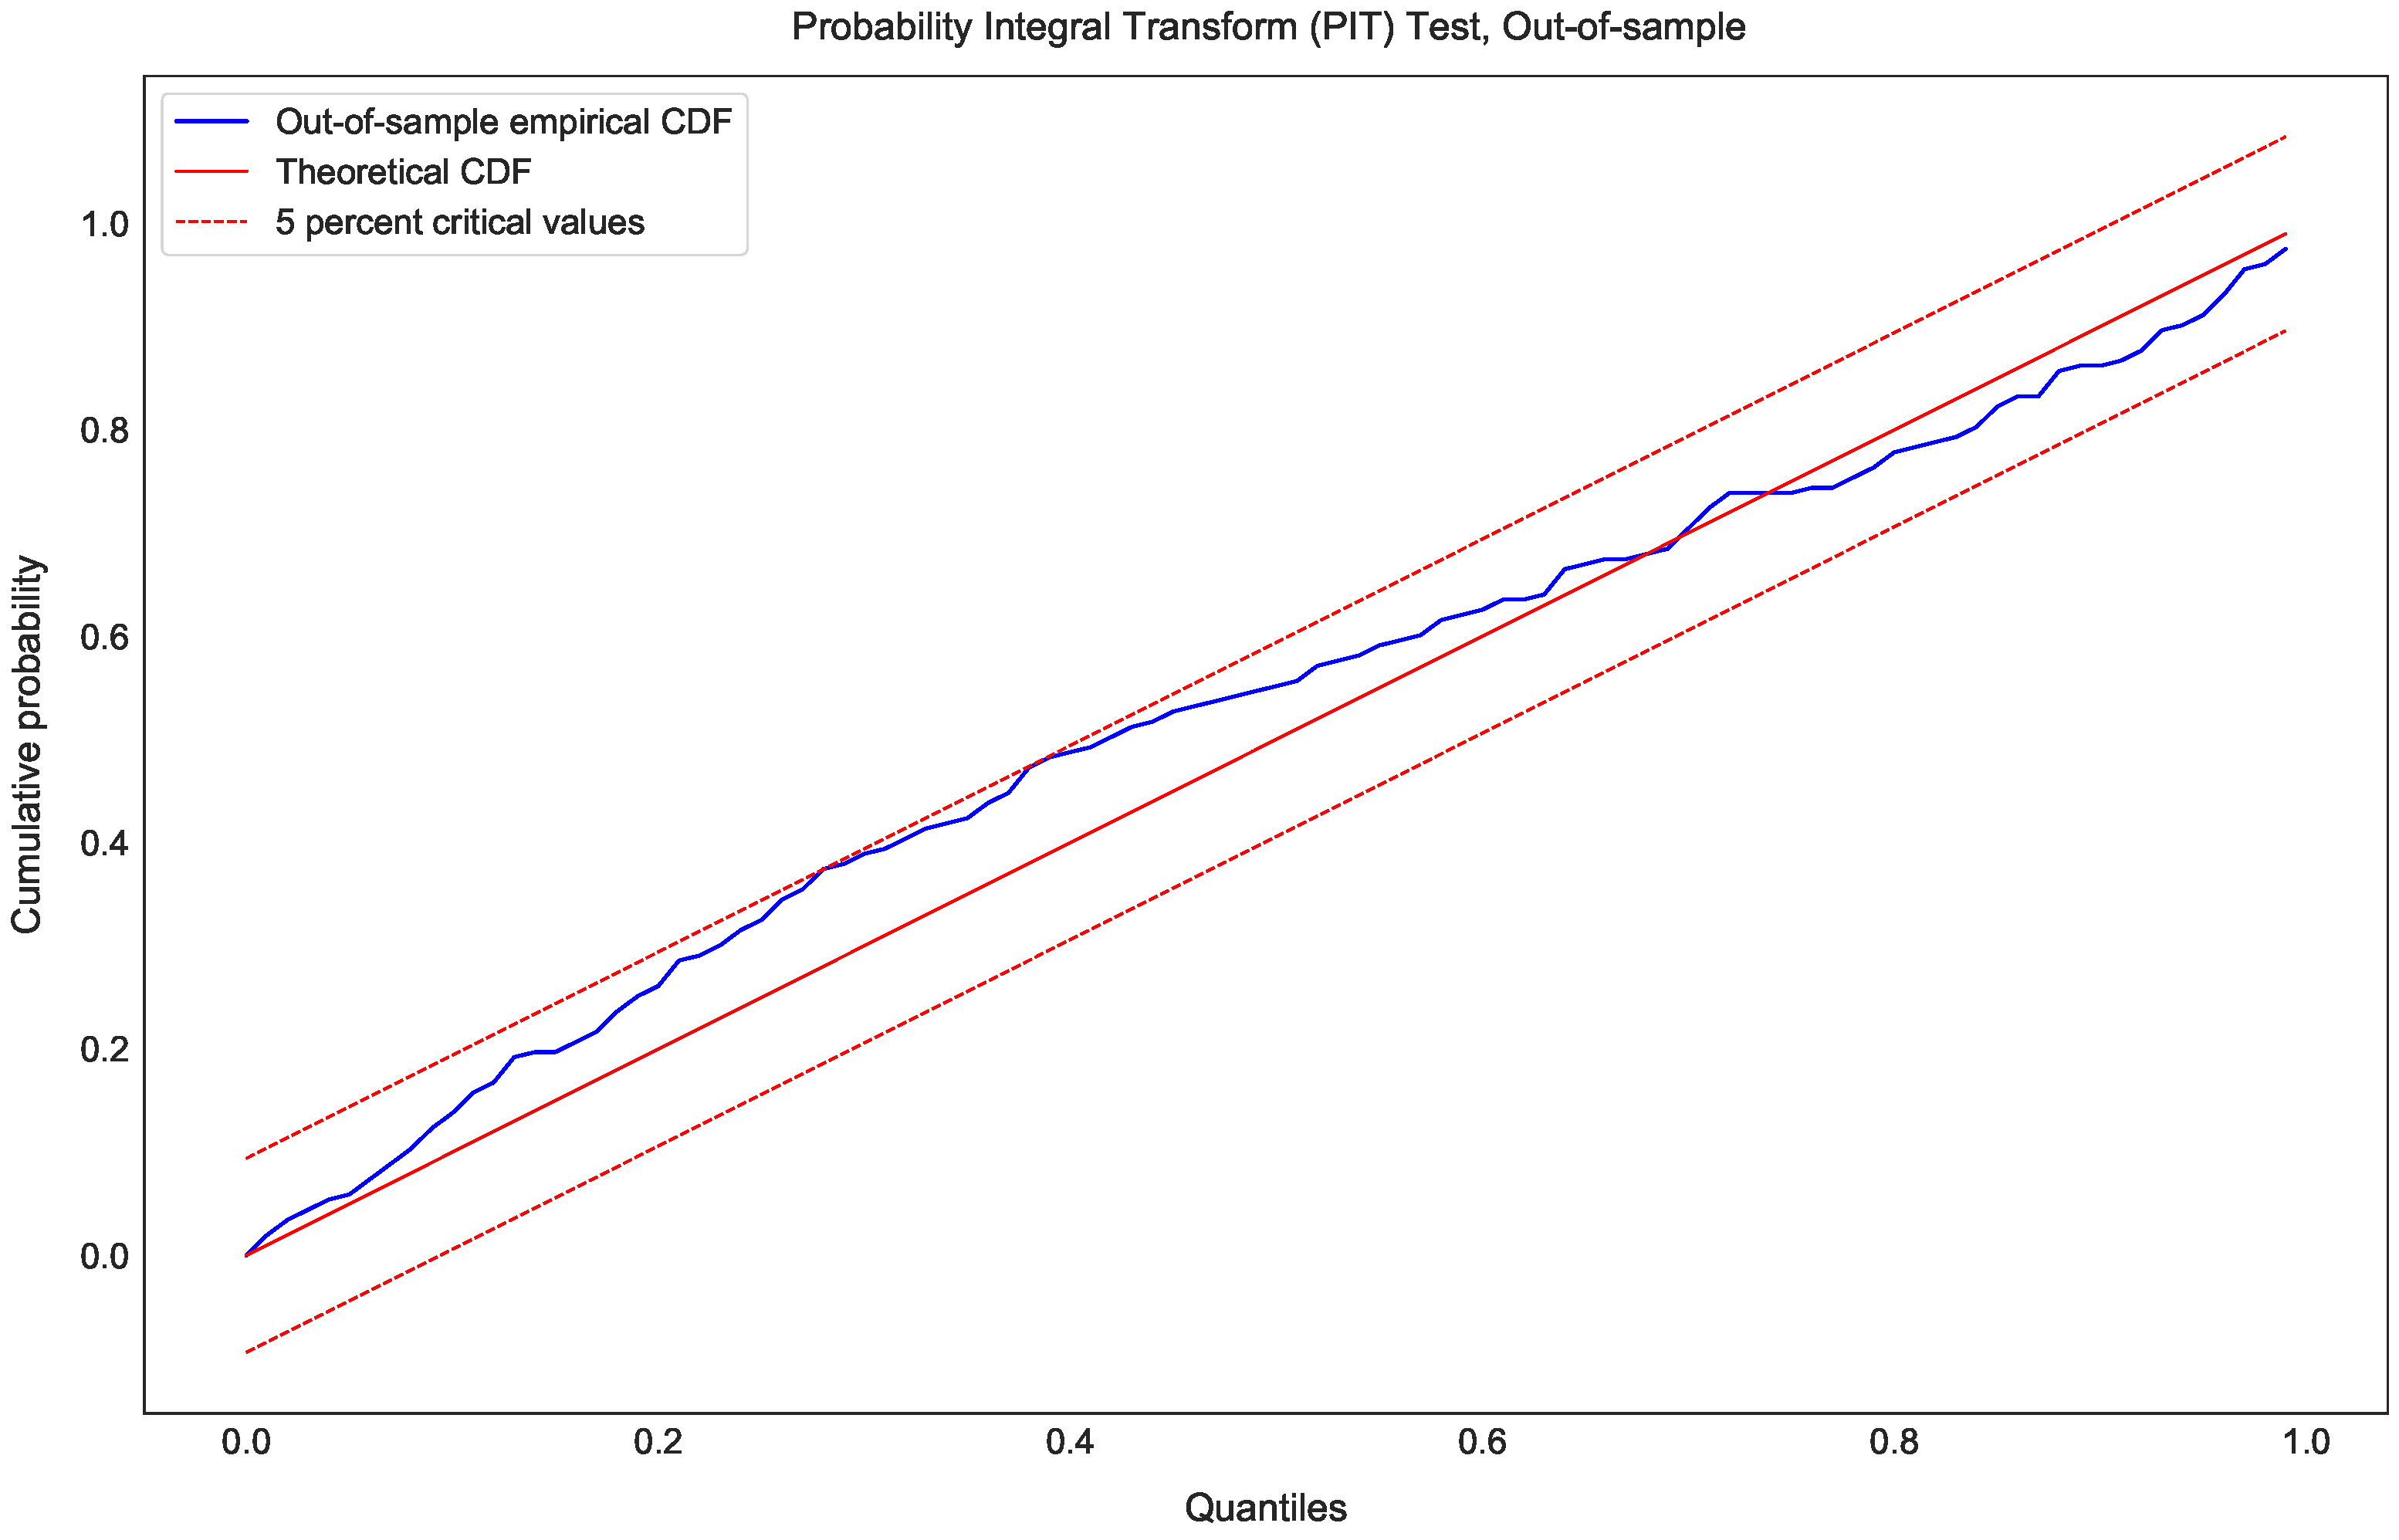
\includegraphics[width=\paperwidth]{pitchart.pdf}}
\end{frame}


%% ---------------------------------------------------------------------------
%% Benchmarking
%% ---------------------------------------------------------------------------
\section{Benchmarking}


\begin{frame}
  \frametitle{Rule-Based Benchmarking: Historical Interventions}
    \makebox[\linewidth]{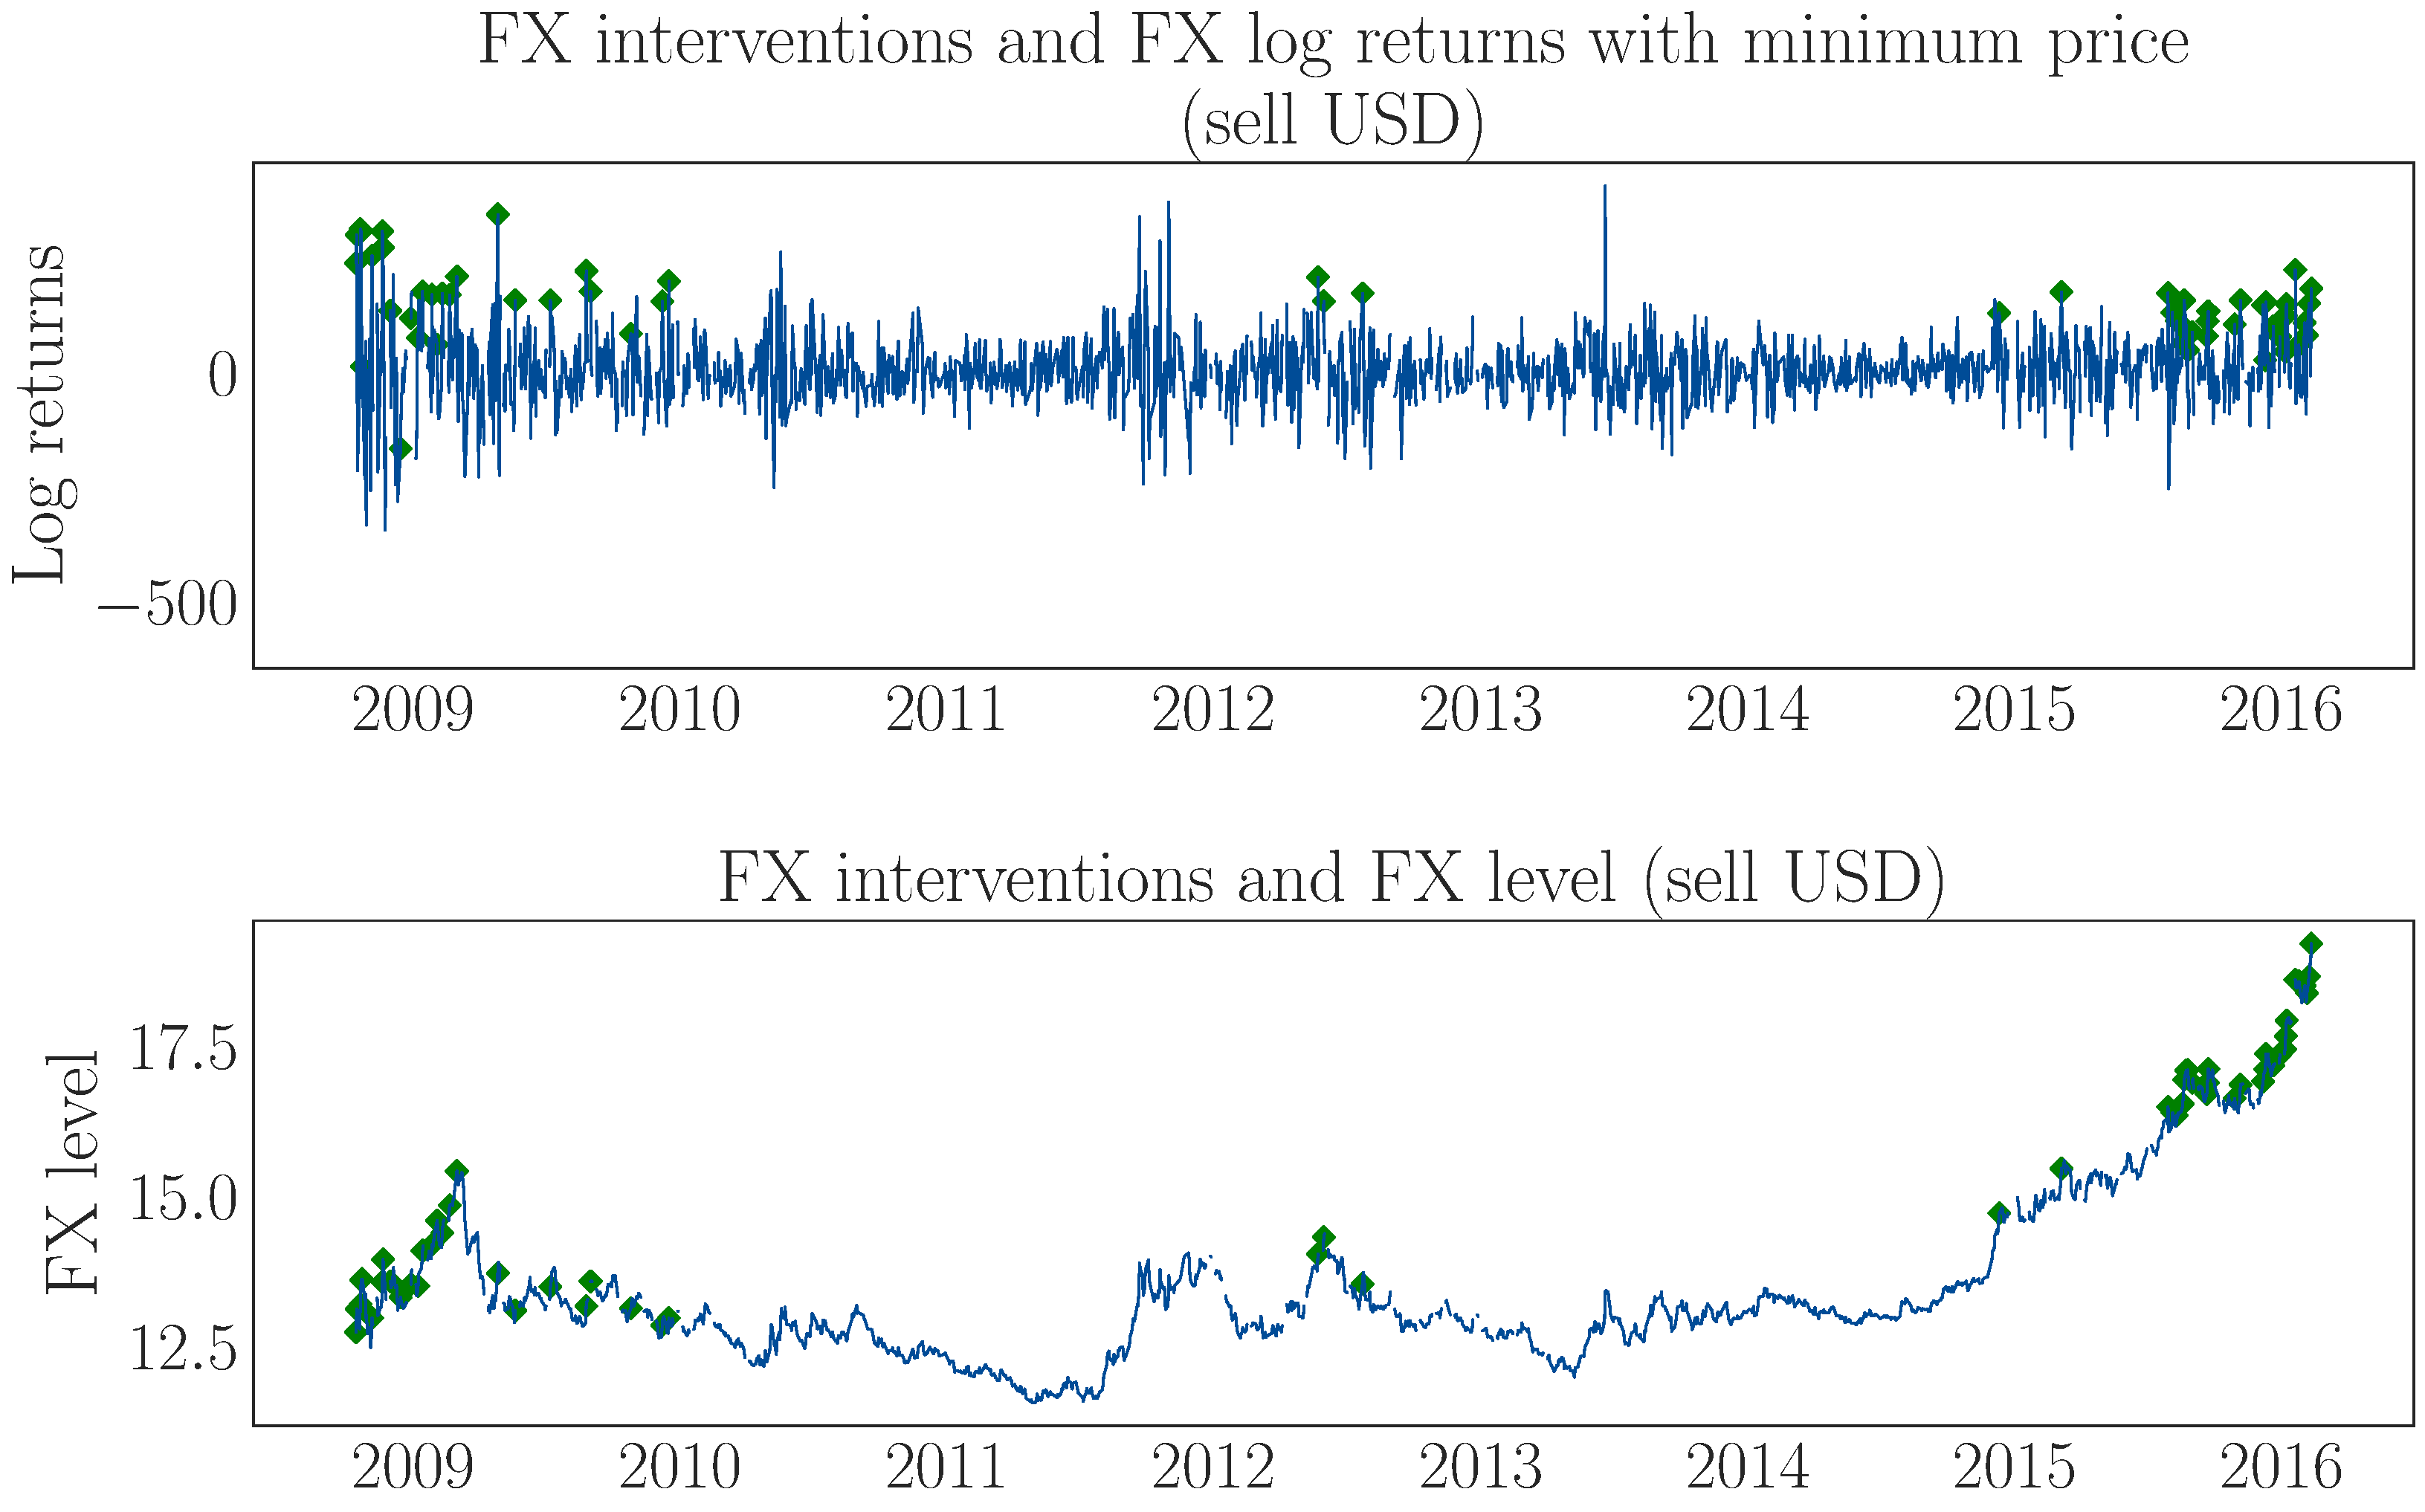
\includegraphics[width=\paperwidth]{benchmark_minprice.pdf}}
\end{frame}


\begin{frame}
  \frametitle{Rule-Based Benchmarking: Risk-Level}
    \makebox[\linewidth]{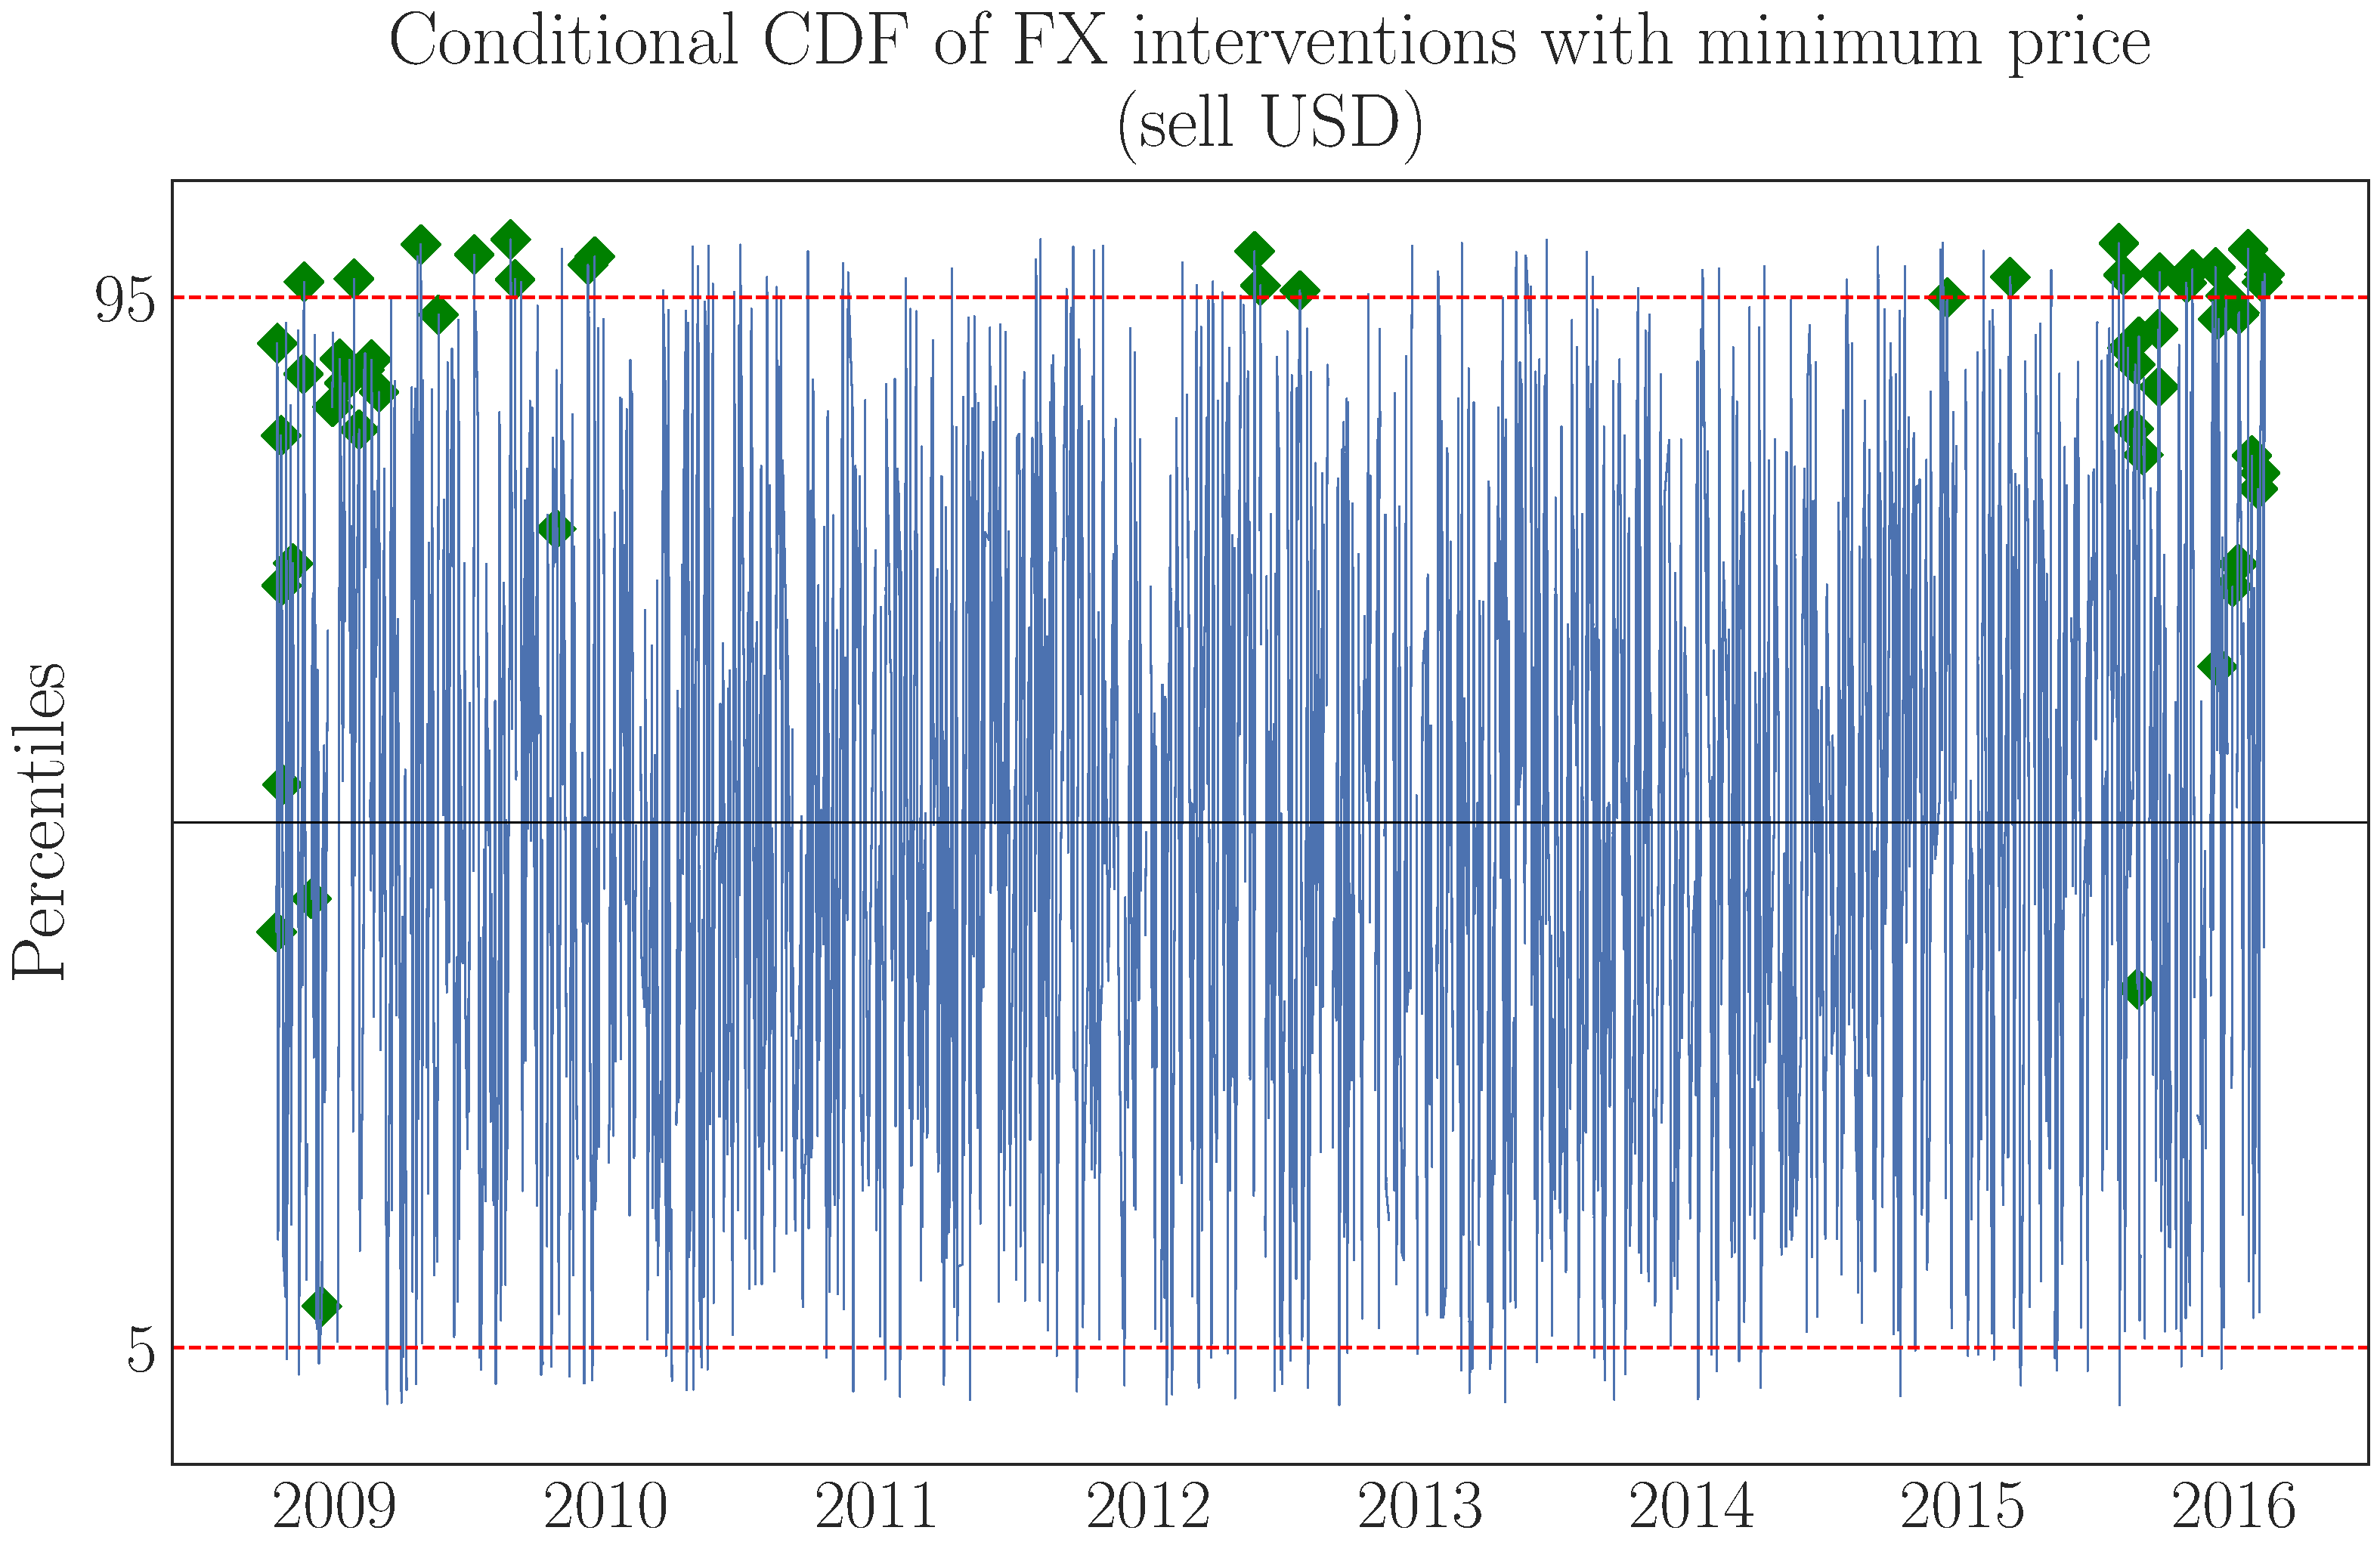
\includegraphics[width=\paperwidth]{benchmark_minprice_cdf.pdf}}
\end{frame}


\begin{frame}
  \frametitle{Discretion-Based Benchmarking: Historical Interventions}
    \makebox[\linewidth]{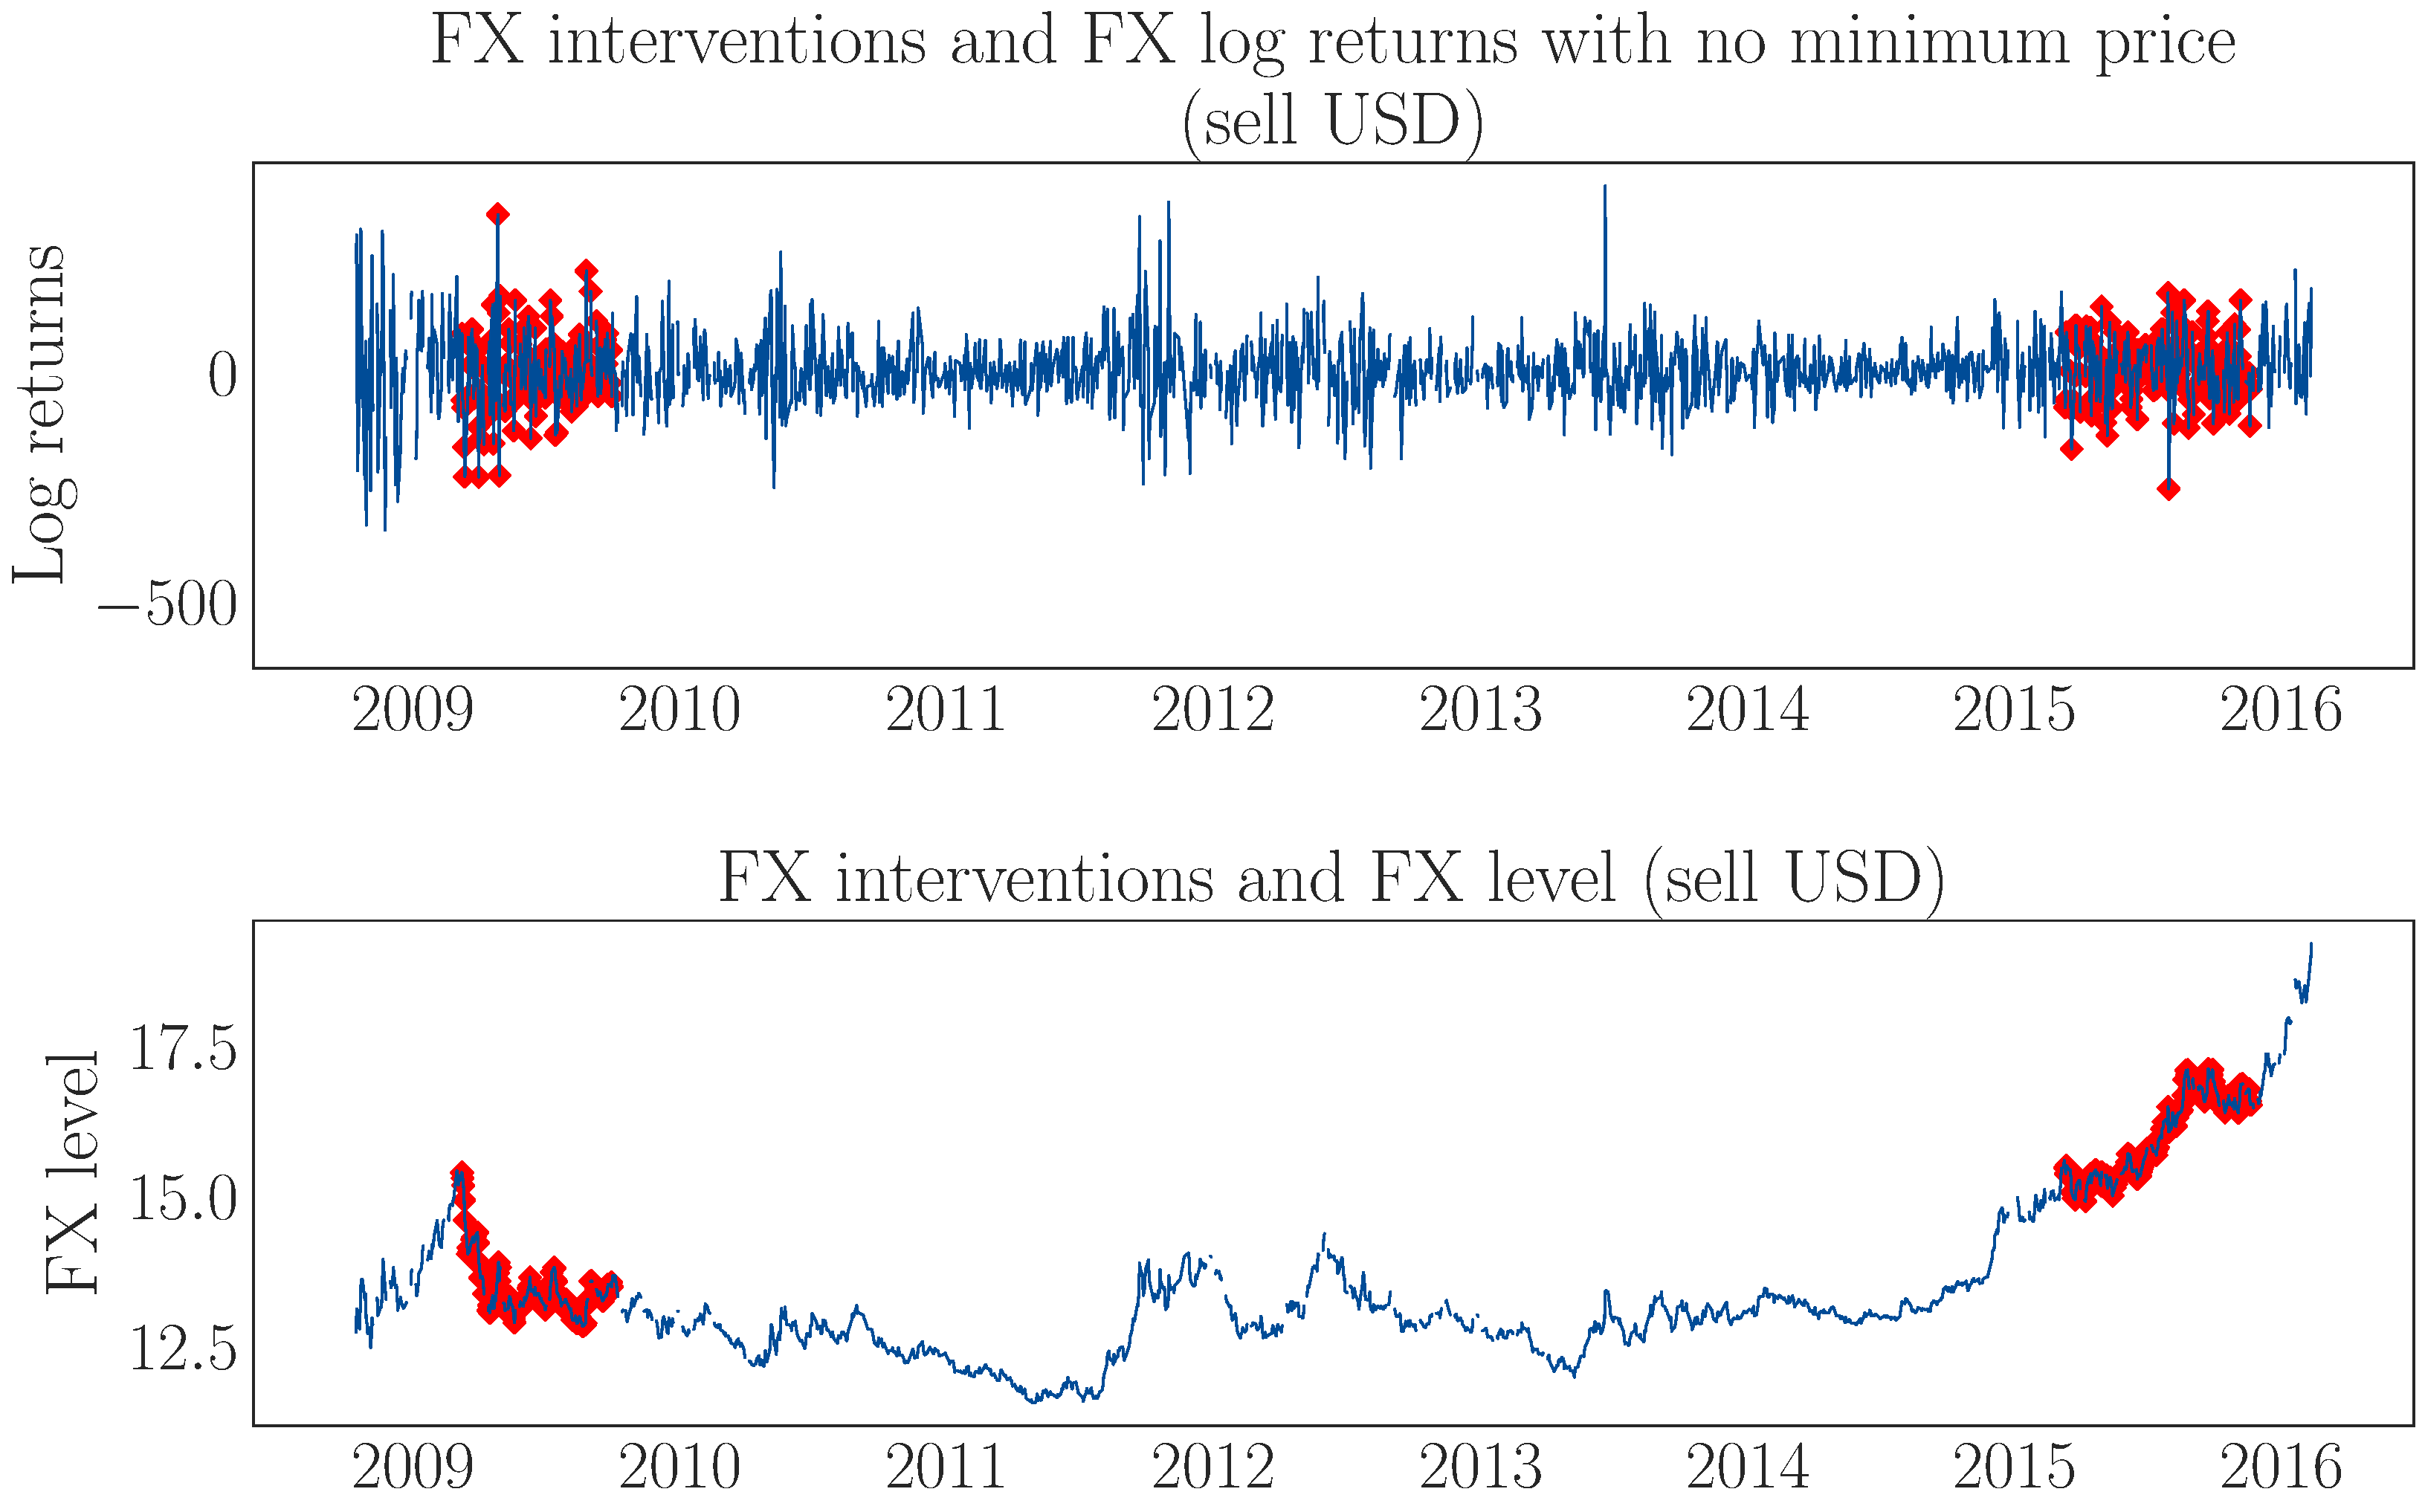
\includegraphics[width=\paperwidth]{benchmark_no_minprice.pdf}}
\end{frame}


\begin{frame}
  \frametitle{Discretion-Based Benchmarking: Risk-Level}
    \makebox[\linewidth]{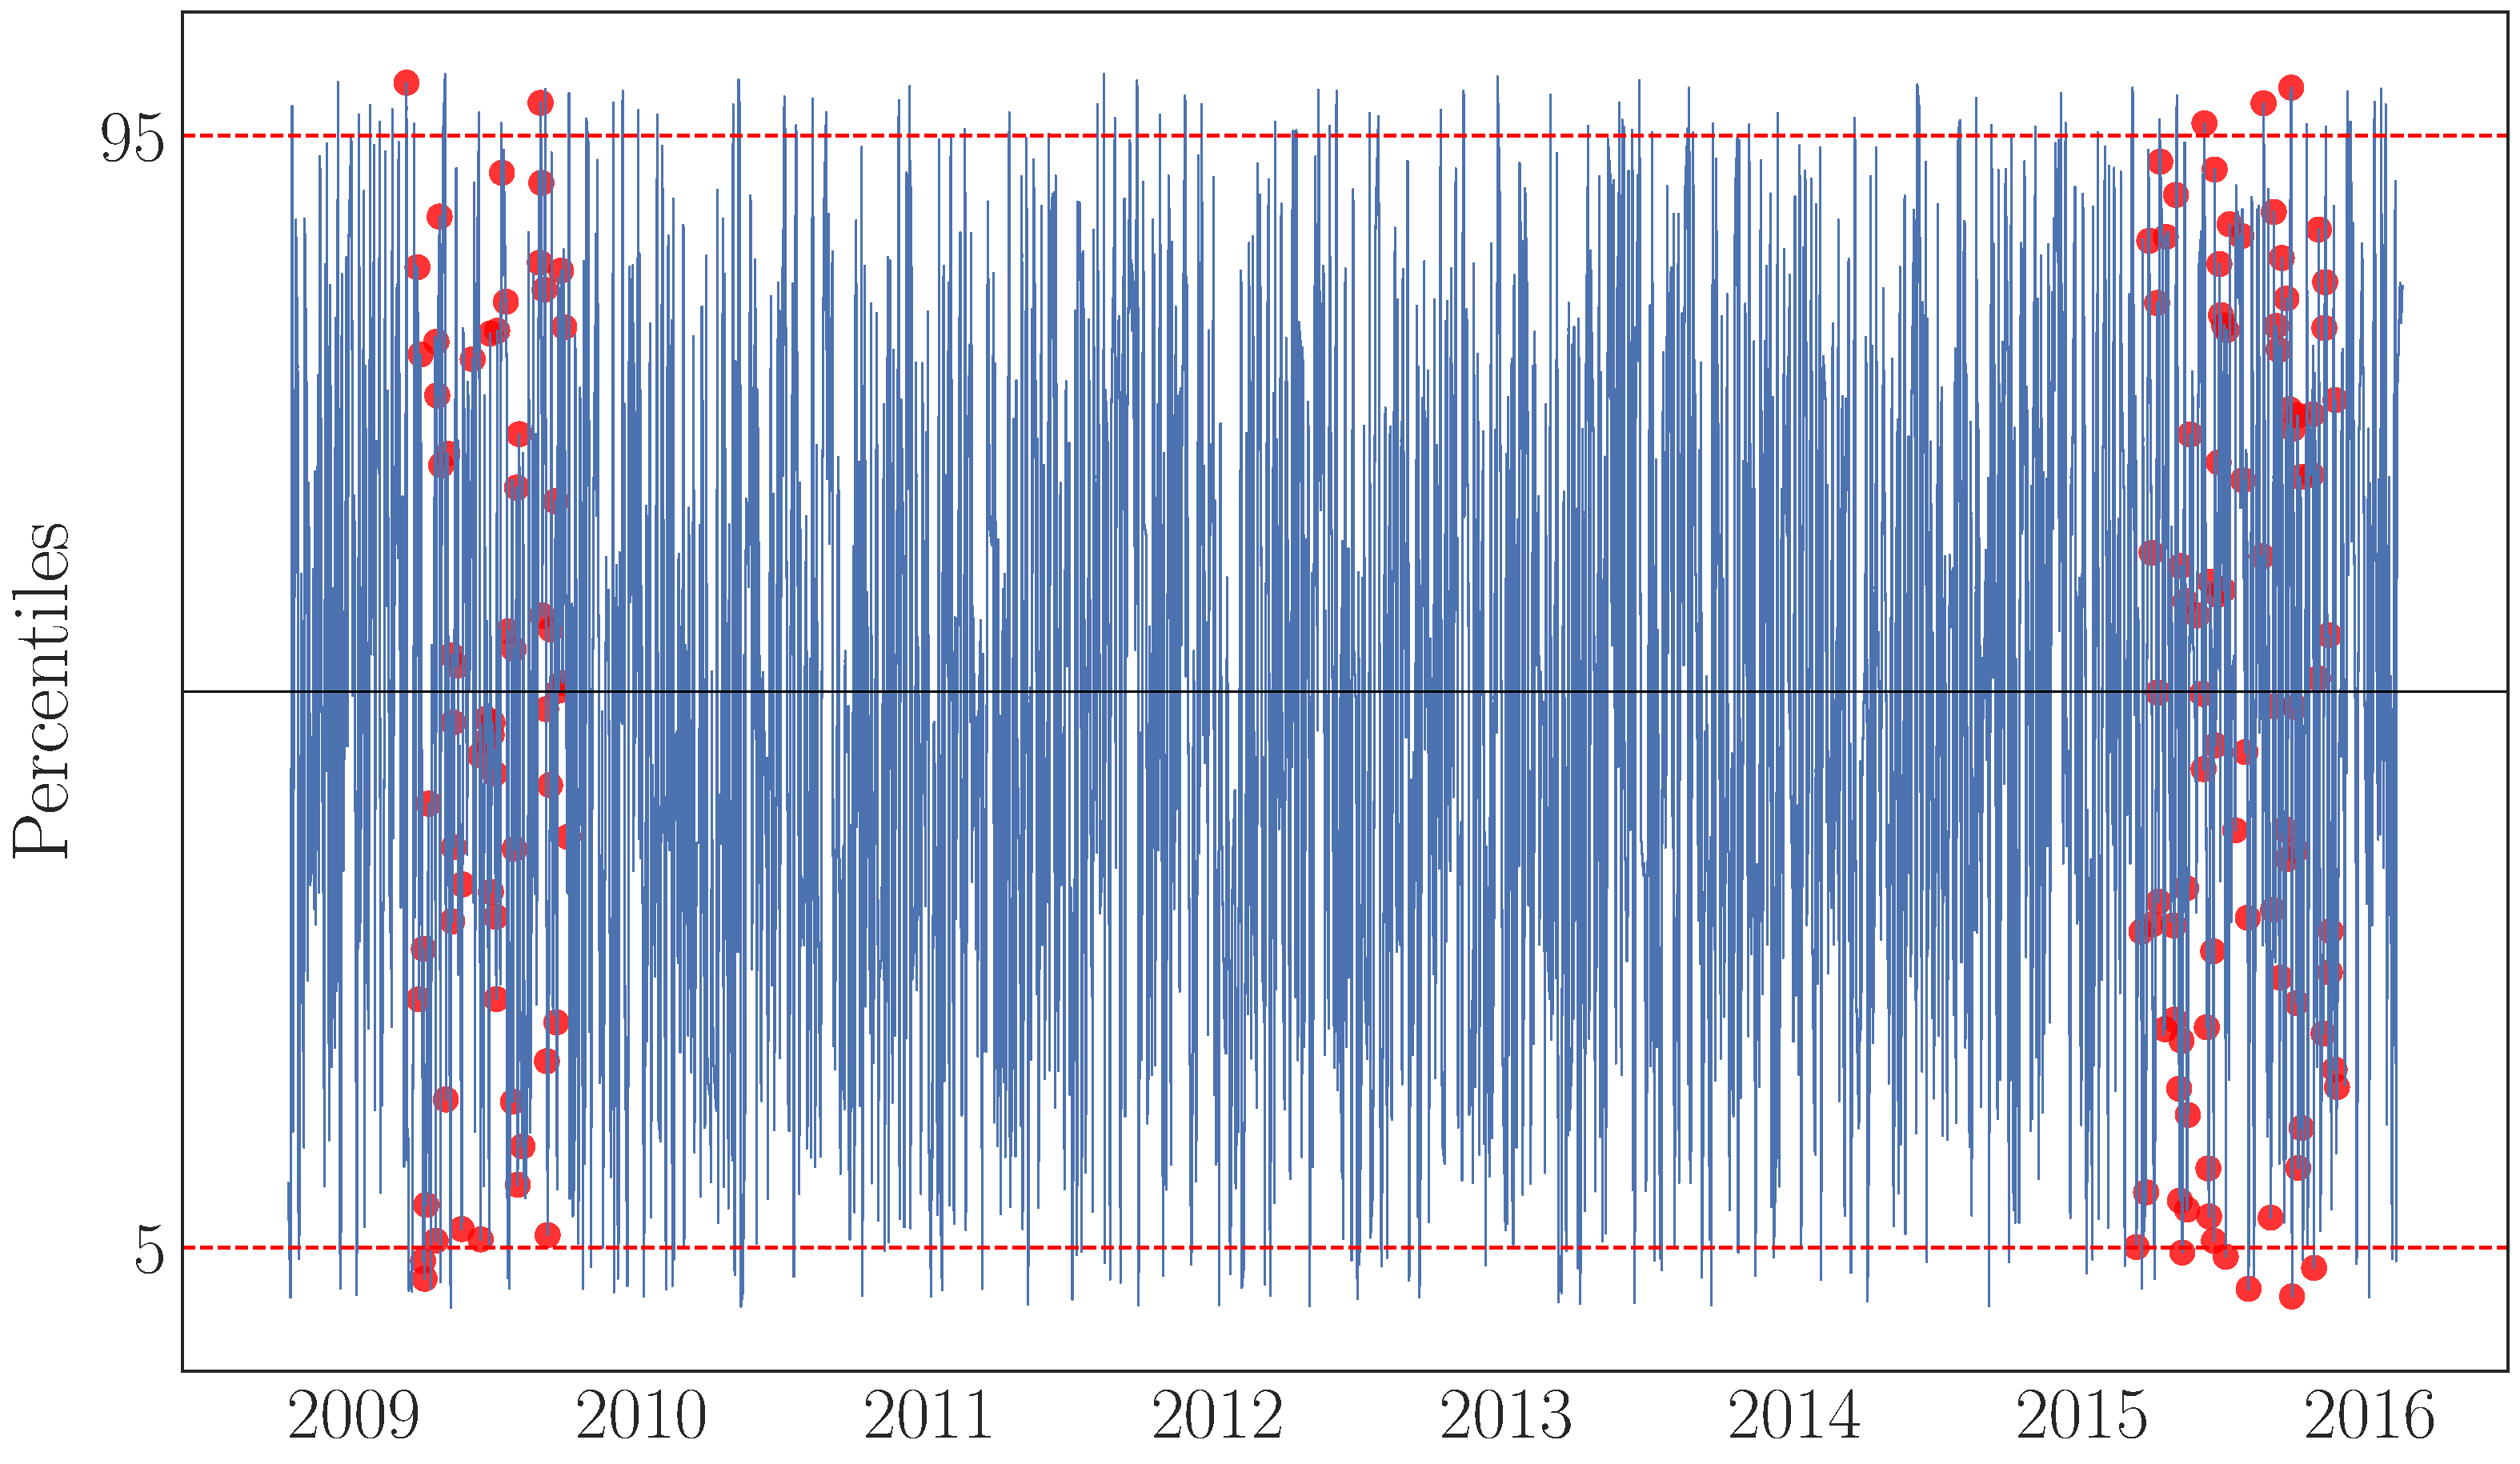
\includegraphics[width=\paperwidth]{benchmark_no_minprice_cdf.pdf}}
\end{frame}




  

%% ---------------------------------------------------------------------------
%% End document
%% ---------------------------------------------------------------------------
\end{document}

